\chapter{Electrostática}

En la naturaliza existen 4 interacciones fundamentales:
\begin{enumerate}
\item Interacción gravitatoria.
\item Fuerza electromagnética.
\item Fuerza nuclear fuerte.
\item Fuerza nuclear débil.
\end{enumerate}

En este curso estudiaremos la segunda, que abarca tanto la fuerza eléctrica como la fuerza magnética.  

Entendemos por \textbf{electromagnetismo} al estudio de los fenómenos eléctricos y magnéticos, los cuales (de forma preliminar) diremos que son producidos por \textit{cargas eléctricas} en reposo o en movimiento.

\myrule{to reversed}{to reversed}

\textbf{Un poco de historia...}

La existencia de la interacción eléctrica fue registrada hace 2.000 años por el griego \textit{Tales de Mileto}, quien observó que un pedazo de ámbar al ser frotado con un un paño, atraía pedacitos de hojas secas. De hecho, la palabra “electricidad” viene del vocablo griego ámbar  (\textbf{elektron}).

\myrule{to reversed}{to reversed}

El electromagnetismo se puede dividir en diferentes ramas tales como: electrostática, circuitería, magnetostática, electrodinámica, \dots

En este capítulo estudiaremos la \textbf{electrostática}, la cual estudia el fenómeno que ocurre cuando las interacciones entre cargas eléctricas están en reposo (o casi).

\section{Carga eléctrica} 

La \textbf{carga eléctrica} es un atributo o propiedad de la materia tan fundamental como la masa, y se hace presente en las partículas  de los átomos constituyentes. 

Existen dos tipos de cargas, las cuales se designan como \textcolor{blue}{positiva} ($+$) y \textcolor{red}{negativa} ($-$). La existencia de estas cargas se observa en el siguiente experimento:

\begin{enumerate}
\item Se frota una barra de vidrio con un paño de seda. 

\item Se frota una varilla de baquelita con un paño de seda.

\begin{figure}[H]
    \centering
    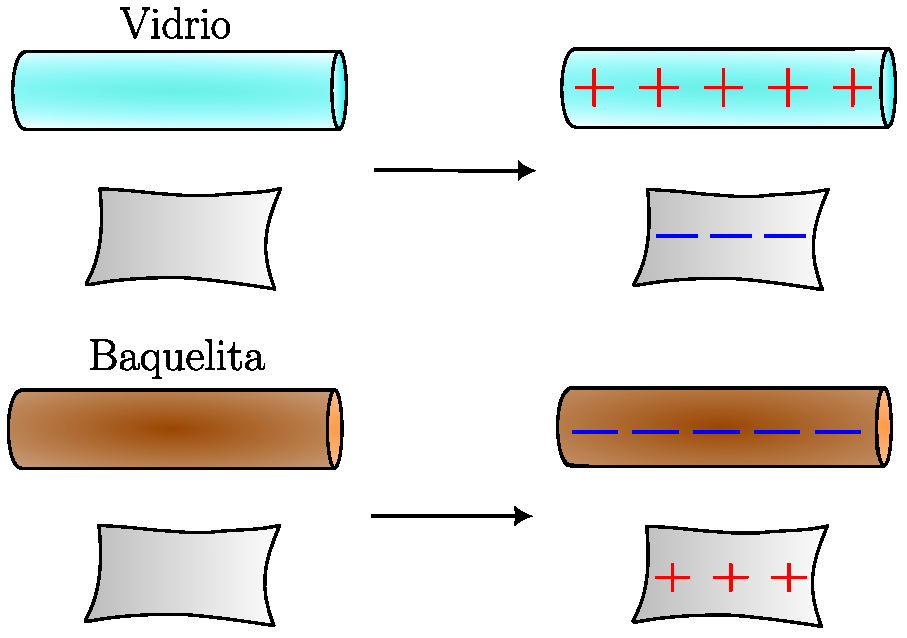
\includegraphics[scale = 0.5]{Figuras/Exp-Carga-Electrico.pdf}
    \caption{La varilla de vidrio queda cargada positivamente al ser frotada con el paño de seda. En cambio la varilla de baquelita queda con carga negativa.}
    \label{fig:Exp-Carga-Electrica1}
\end{figure}

\item Suspendemos la barra de vidrio cargada con un cordón, ver figura \ref{fig:Exp-Carga-Electrica2}-(a), y colocamos cerca una segunda barra de vidrio cargada, observamos que las dos barras se repelen entre sí. Sin embargo, si acercamos la varilla de baquelita, ésta atrae al extremo de la barra de vidrio suspendida, ver figura \ref{fig:Exp-Carga-Electrica2}-(b).

\end{enumerate}

Para poder explicar este resultado se propuso  que la barra de vidrio queda cargada y llamamos a esta carga \textit{positiva}. De igual manera queda cargada la varilla de baquelita y llamamos a esta carga \textit{negativa}.

Así, el paso 3. comprueba un importante principio:

\colorlet{shadecolor}{blue!10}
\begin{shaded}
\begin{center}
\textit{Cargas iguales se repelen y cargas distintas se atraen.}
\end{center}
\end{shaded}
\colorlet{shadecolor}{green!20}

\textbf{¿Pero cuál es el origen de la carga eléctrica?}

La materia está constituida de átomos. Cada átomo consiste de un núcleo, que contiene protones y neutrones, y este núcleo está rodeado por un cierto número de electrones. Los electrones tienen carga \textcolor{blue}{negativa} y los protones \textcolor{red}{positiva}, y los neutrones NO tienen carga eléctrica \footnote{No es adecuado decir carga cero o neutra.}. Los electrones pueden ser extraídos de los átomos mucho más fácilmente que los protones y neutrones. Por ello, el número de protones en el núcleo atómico determina la identidad de los elementos químicos.

La fuerza de repulsión o atracción entre dos cuerpos cargados dependerá de la  “cantidad neta de carga” que posean. Por carga neta se entiende la carga en exceso (positiva o negativa) que un cuerpo posee comparado con el mismo cuerpo neutro. Si se separan uno o más electrones, la estructura restante con carga positiva es un \textbf{ión positivo}. En el caso contrario que el átomo haya ganado uno o más electrones es un \textbf{ión negativo}. Esta ganancia o pérdida de electrones se conoce como \textbf{ionización}.

\begin{figure}[H]
    \centering
    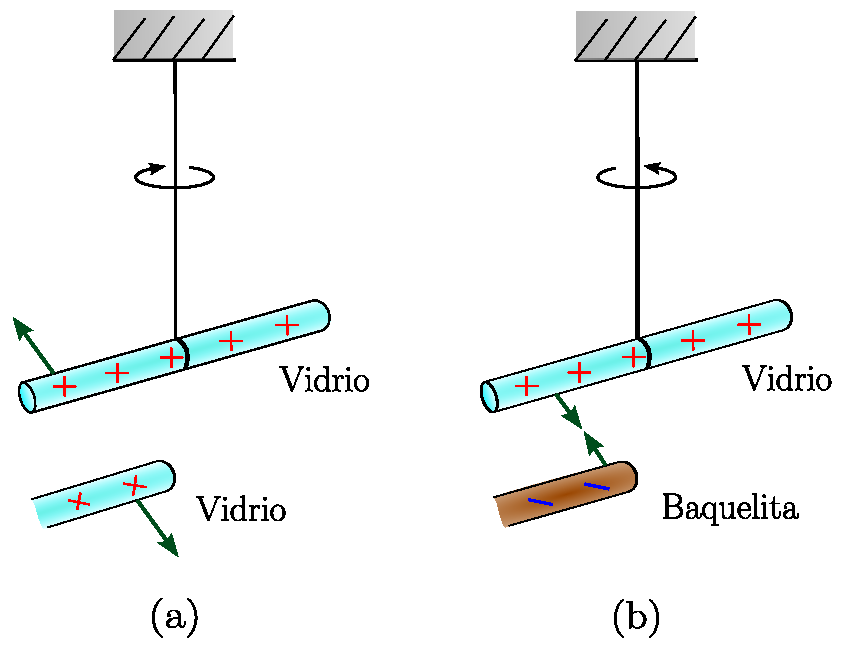
\includegraphics[scale = 0.7]{Figuras/Cargas-Opuestas-Iguales.pdf}
    \caption{(a) Dos varillas con cargas iguales se repelen entre sí. (b) Dos varillas con cargas opuestas se atraen mutuamente.}
    \label{fig:Exp-Carga-Electrica2}
\end{figure}

\subsection{Principios}

\subsubsection{Principio de cuantización de la carga}

Los experimentos demuestran además que la carga está \textbf{cuantizada}. Ésto quiere decir que la carga viene en múltiplos enteros de una carga elemental ($e$). En otras palabras, si un cuerpo tiene una carga neta $q$, entonces necesariamente se cumple:
\begin{equation*}
\boxed{q = \pm N e}
\end{equation*}

donde $N \in \mathbb{N}$ y $e$ es la \textbf{carga fundamental} que tiene un valor de \cite{CODATA}
\begin{equation*}
e = 1.602 176 634 \times 10^{-19} \, [C],
\end{equation*}

donde la unidad de carga es llamada \textbf{Coulomb} ($C$). Para nuestro caso, utilizaremos el valor $e = 1.602 \cdot 10^{-19} \, [C]$. Esto quiere decir que NO puede haber una carga más pequeña que $e$, la cual corresponde al valor absoluto de la carga del electrón.

\textbf{Observación:} La unidad de medida de la carga en el S.I es el Amperè segundo $[A\,s]$, donde $1 \, \mbox{Coulomb} \, = \,1 \,\mbox{Amperè\,segundo}$ y $1 \,[A] = 6.24150962915265 \cdot 10^{18}$ cargas elementales por segundo. Es decir, son necesarios $6 \times 10^{18}$ electrones para completar una carga de $-1.0 \,[C]$!!!

Para darse una idea del tamaño de las partículas que constituyen un átomo, se muestran en la tabla: las masas de los electrones, protones y neutrones junto con sus respectivas cargas \cite{Alvarez}. 

\begin{center}
 \begin{tabular}{ccc}
 \hline
 Partícula & Masa (kg) & Carga (C) \\ \hline
 electrón &   $9.11 \times 10^{-31}$ & $- 1.602 \times 10^{-19} ~ (-e)$ \\
 protón & $1.673 \times 10^{-27}$ & $+ 1.602 \times 10^{-19} ~(+e)$ \\
 neutrón & $1.675 \times 10^{-27}$ &  --- \\
 \hline 
 \end{tabular}
\end{center}

Se puede apreciar que $m_{\text{núcleo}} \approx 2.000 \, m_e$, es decir, el $99 \%$ de la masa del átomo es su núcleo. Además, la magnitud de la carga del electrón o del protón, en valor absoluto, son iguales.

\subsubsection{Principio de conservación de la carga}

Este principio establece que la carga neta de un sistema \textit{aislado} permanece constante, es decir,
\begin{equation*}
\sum_i q_i = cte.
\end{equation*}

Si un sistema parte con un número igual de cargas positivas y negativas, no se puede hacer nada para crear un exceso de carga negativa o positiva en el sistema a menos que traigamos una carga desde afuera del sistema (o quitar alguna carga del sistema).

\subsection{Tipos de materiales}

Las fuerzas entre dos objetos cargados pueden ser muy grandes. La mayoría de los objetos son eléctricamente neutros; tienen igual cantidad de cargas positivas que negativas.

Los materiales están divididos en tres categorías, dependiendo cuan fácilmente permiten el flujo de carga (ej. electrones) a lo largo de ellos. Éstos son:

\begin{itemize}
\item Los \textbf{Conductores} son cuerpos que, aunque estén neutros, tienen una enorme cantidad de \textit{electrones libres}, es decir, no ligados a los átomos, aptos para conducir la electricidad. Obviamente, la carga de estos electrones es neutralizada por la de los protones nucleares que están en los núcleos que supondremos fijos.

\textbf{Ejemplo:} Los metales y los electrolitos.

\item Los \textbf{aisladores} no conducen la electricidad ya que no poseen cargas libres, pero sus moléculas pueden polarizarse bajo influencia de una interacción eléctrica externa. Que se polaricen significa que estas moléculas, aunque neutras, pueden deformarse y/o orientarse, en mayor o menor grado. Esto confiere a los aisladores las denominadas \textit{propiedades dieléctricas} que estudiaremos después.

\textbf{Ejemplo:} Goma, madera, cerámica, plástico, \dots

\item Los \textbf{semiconductores}, que son la base de la electrónica actual, son cuerpos con propiedades de conducción intermedias entre los conductores y aisladores. En ellos se puede variar, con relativa facilidad, el número de cargas libres o portadores de electricidad.

\textbf{Ejemplo:} El silicio y el germanio.
\end{itemize}

\subsection{Métodos para cargar un objeto}

Hay tres maneras de cargar un objeto. 

\begin{enumerate}
\item Por \textbf{frotamiento}: esto es útil para cargar aisladores. Al comienzo de la sección se mostró un ejemplo de este método.

\item Por \textbf{conducción}: es útil para cargar metales y otros conductores. Si un objeto cargado toca a un conductor, una cantidad de carga será transferida entre el objeto y el conductor, de tal manera que el conductor quedará cargado con el mismo signo que la carga del objeto.

\item Por \textbf{inducción}: también es útil para cargar metales y otros conductores. 

 \textbf{Por ejemplo:} Acerquemos, sin tocar, una barra cargada negativamente a una esfera metálica neutra y aislada. Las cargas en la esfera se polarizan, es decir, los electrones se acumulan en un lado de la esfera, y del otro lado se produce deficiencia de electrones (carga +), pero la esfera sigue siendo neutra. Después, se conecta un alambre que permite que los electrones acumulados fluyan a tierra \footnote{ La Tierra es un conductor, y es tan
grande que actúa como una fuente prácticamente infinita de electrones adicionales o como un receptor de los electrones no deseados.}. Se desconecta el alambre de la esfera y se retira la barra con carga. Los electrones de la esfera se redistribuyen: la esfera en conjunto tiene una deficiencia de electrones (carga $+$), ver figura \ref{fig:Induccion-1}. 

En forma análoga, si se acerca una barra
cargada positivamente, se produce al final una esfera cargada negativamente,  ver figura \ref{fig:Induccion-2}.

\begin{figure}[H]
    \centering
    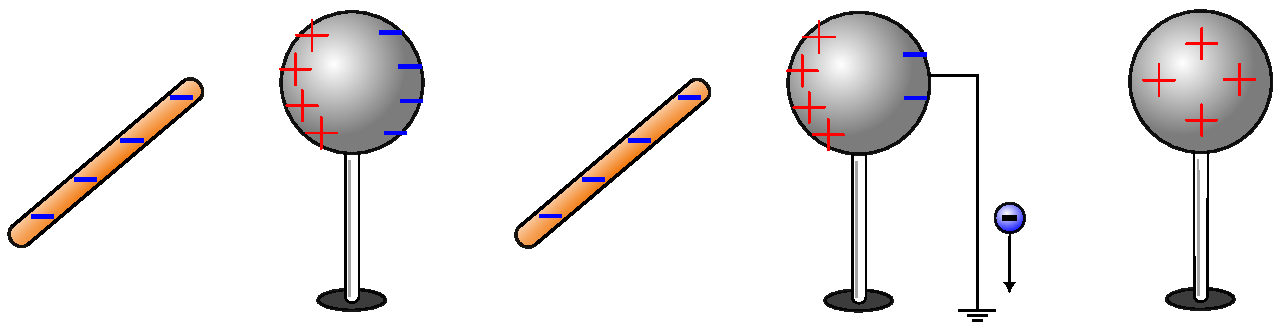
\includegraphics[scale = 0.5]{Figuras/Induccion-1.pdf}
    \caption{Inducción eléctrica, se acerca una barra con carga negativa a una esfera metálica, después de la conexión a tierra la esfera queda cargada positivamente.}
    \label{fig:Induccion-1}
\end{figure}

\begin{figure}[H]
    \centering
    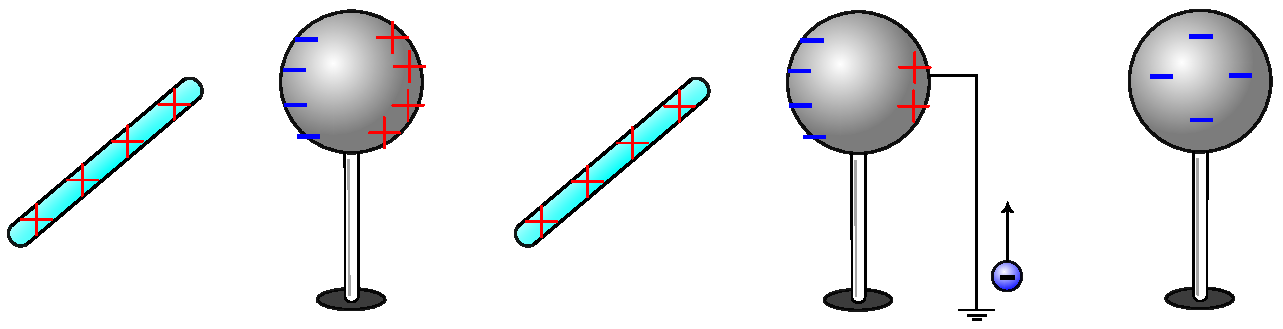
\includegraphics[scale = 0.5]{Figuras/Induccion-2.pdf}
    \caption{Inducción eléctrica, se acerca una barra con carga positiva a una esfera metálica, después de la conexión a tierra la esfera queda cargada negativamente.}
    \label{fig:Induccion-2}
\end{figure}
\end{enumerate}

\section{Ley de Coulomb}

\textbf{Charles Augustin Coulomb} (1736-1806) estudió en detalle, en 1785, las fuerzas de interacción de las partículas con carga eléctrica, utilizando una \textit{balanza de torsión} de Cavendish.

La \textit{balanza de torsión} consiste en una barra liviana colgada en su centro por un alambre de cuarzo (fibra de torsión) cuya constante elástica torsional $K$ se conoce, ver figura \ref{fig:Balanza-Torsion}.
En los extremos de la barra existen esferas de igual masa. Solo una de ellas posee carga eléctrica $q_1$, la cual se enfrenta a otra de carga eléctrica de igual signo $q_2$, fija en el laboratorio. 

Recordemos de los primeros cursos de Física que cuando una barra o varilla rota un ángulo $\theta$ a partir de su posición de equilibrio (en una balanza de torsión), el alambre se tuerce ejerciendo sobre la varilla un torque alrededor del centro que se opone al desplazamiento $\theta$ y de magnitud proporcional al ángulo, $\tau = K \theta$ (en magnitud), donde $K$ es la constante elástica de torsión. Luego de haber alcanzado el equilibrio rotacional, según los datos de la figura \ref{fig:Balanza-Torsion}-(b), se verifica que
$$Fb = K \theta \Rightarrow F = \frac{K\theta}{b},$$

donde $F b$ es el torque generado por la fuerza que ejerce la carga $q_2$ sobre $q_1$ con $b$  la distancia a la que se encuentra el punto $O$ de la recta de aplicación de la fuerza.

Experimentando con diferentes cargas y diferentes longitudes de barra, Coulomb encontró que para cargas puntuales, la magnitud de cada una de las fuerzas eléctricas con que interactúan 2 cargas puntuales es directamente proporcional al producto de las cargas e inversamente proporcional al cuadrado de la distancia que los separa con dirección según la linea que los une.
$$F \propto \frac{|q_1q_2|}{r^2} ~\Rightarrow ~ F = k \frac{|q_1q_2|}{r^2}.$$

El valor de la constante de proporcionalidad $k$ depende del sistema de unidades que se utilice. En el S.I.,
$$k = 8.987551787 \times 10^9 \,[Nm^2/C^2] \approx 9 \times 10^9 \, [Nm^2/C^2].$$

La constante $k$ se suele escribir como:
$$k = \frac{1}{4\pi \varepsilon_0}.$$

Luego, la \textbf{ley de Coulomb} se puede expresar de la siguiente manera
$$\boxed{F = \frac{1}{4\pi\varepsilon_0} \frac{|q_1q_2|}{r^2}}$$

donde las cargas están dadas por $q_1$ y $q_2$, la distancia de separación por $r$ y $\varepsilon_0 = 8.854 \times 10^{-12} \,[C^2/Nm^2]$ es la \textbf{permitividad eléctrica del espacio vacío} \cite{CODATA}.
\begin{figure}
        \centering
        \subfigure[]{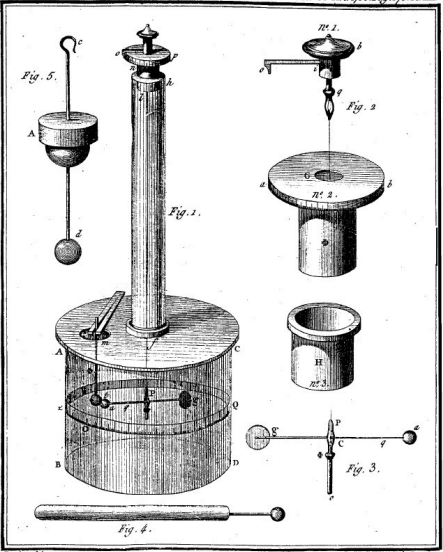
\includegraphics[width=0.5\textwidth]{Figuras/Exp_Coulomb.png}} \hspace{1cm}
        \subfigure[]{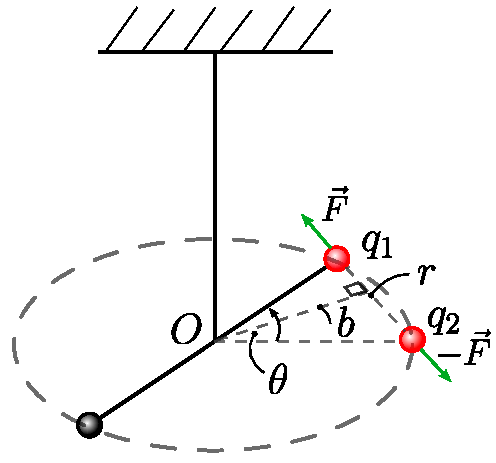
\includegraphics[width=0.4\textwidth]{Figuras/Esquema-Exp-Coulomb.pdf}} 
        \caption{En (a), el diagrama de la balanza de torsión de Coulomb. Recuperado de: Coulomb, C. A. (1788). \textit{Sur l'électricité et le magnétisme, premier mémoir}. En: Mémoires de l'Academie Royale des Sciences pour l’année 1785, Paris, pág 576. En (b), un dibujo esquemático de la balanza de torsión.}
        \label{fig:Balanza-Torsion}
    \end{figure}


\subsection*{Carácter vectorial}

Sean dos cargas puntuales, $q_1$ y $q_2$ en el vacío,  ubicadas mediante los
vectores posición $\vec{x}_1$ y $\vec{x}_2$ respecto a un sistema de referencia.

\begin{figure}[H]
    \centering
    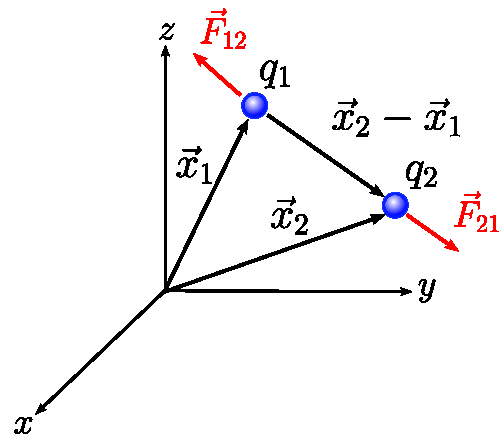
\includegraphics[scale = 0.7]{Figuras/Coulomb-Vectorial.pdf}
    \caption{Posición de las cargas puntuales.}
    \label{fig:Coulomb-Vectorial}
\end{figure}

 La ley de Coulomb establece que la fuerza que actúa sobre una partícula cargada $q_1$ debido a otra partícula cargada $q_2$ es:
 \begin{equation*}
 \vec{F}_{12} = \underbrace{\frac{1}{4\pi \varepsilon_0} \frac{q_1 q_2}{|\vec{x}_1 - \vec{x}_2|^2}}_{\text{Magnitud}} \underbrace{\frac{\vec{x}_1 - \vec{x}_2}{|\vec{x}_1 - \vec{x}_2|}}_{\text{Vector unitario}} = \frac{1}{4\pi \varepsilon_0} \frac{q_1 q_2}{|\vec{x}_1 - \vec{x}_2|^3} (\vec{x}_1 - \vec{x}_2).
 \end{equation*}

Análogamente, la fuerza que actúa sobre la partícula $q_2$ debido a otra
partícula cargada $q_1$ es:
\begin{equation*}
 \vec{F}_{21} = \underbrace{\frac{1}{4\pi \varepsilon_0} \frac{q_1 q_2}{|\vec{x}_2 - \vec{x}_1|^2}}_{\text{Magnitud}} \underbrace{\frac{\vec{x}_2 - \vec{x}_1}{|\vec{x}_2 - \vec{x}_1|}}_{\text{Vector unitario}} = - \frac{1}{4\pi \varepsilon_0} \frac{q_1 q_2}{|\vec{x}_1 - \vec{x}_2|^3} (\vec{x}_1 - \vec{x}_2).
 \end{equation*}

Note que se obedece la \textit{tercera ley de Newton}:
\begin{equation*}
\vec{F}_{12} = - \vec{F}_{21}. 
\end{equation*}

\textbf{Observación:} La ley de Coulomb para distancias muy cortas falla pues $F \to \infty$ cuando $r \to 0$. Si ésto es cierto, no existiría los núcleos atómicos.

\begin{ejemplo}
Calcule la fuerza que actúa sobre la carga $q_1 = -1,0 \times 10^{-6} \,[C]$ ubicada en el punto $(5,5) \,[cm]$ de un sistema cartesiano, y que es ejercida por una carga puntual $q_2 = 2,0 \times 10^{-6} \, [C]$, fija en el punto $(1,2) \,[cm]$. 


\begin{figure}[H]
    \centering
    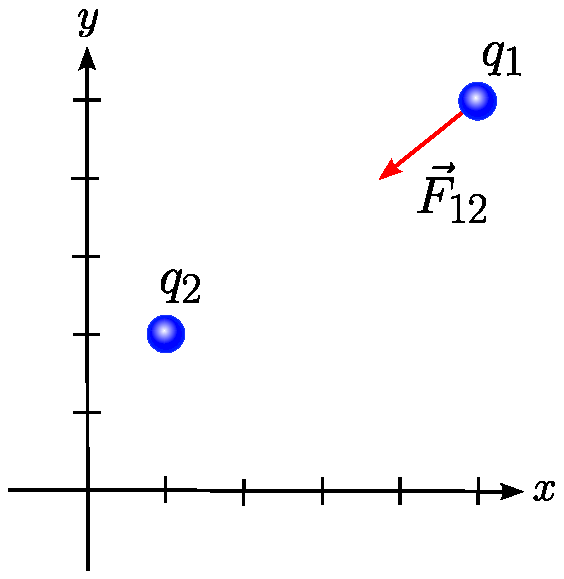
\includegraphics[scale = 0.5]{Figuras/Ej-Coulomb.pdf}
    \caption{Esquema.}
    \label{fig:Ej-Coulomb}
\end{figure}

\textbf{Solución:} Primero, se tiene que $\vec{x}_1 = (5 \,\hat{\imath} + 5 \, \hat{\jmath}) \,[cm]$ y $\vec{x}_2= (  \hat{\imath} + 2 \,\hat{\jmath}) \,[cm]$. Luego,
\begin{align*}
 \vec{x}_1 - \vec{x}_2 &= (5 \,\hat{\imath} + 5 \,\hat{\jmath}) - (\hat{\imath} + 2 \, \hat{\jmath}) \,[cm] = (4 \,\hat{\imath} + 3\,\hat{\jmath}) \,[cm] = (0.04 \,\hat{\imath} + 0.03\,\hat{\jmath}) \,[m], \\
|\vec{x}_1 - \vec{x}_2|^3 &= \left( \sqrt{4^2 + 3^2} \right)^3 = 125 \,[cm^3] = 1.25 \times 10^{-4} \, [m^3].   
\end{align*}

Entonces,
\begin{align*}
    \vec{F}_{12} &= k \frac{q_1q_2}{|\vec{x}_1 - \vec{x}_2|^3} (\vec{x}_1 - \vec{x}_2) \\
&= (9 \times 10^9) \cdot \frac{(-1\times 10^{-6})(2\times 10^{-6})}{1.25 \times 10^{-4}} (0.04 \,\hat{\imath} + 0.03 \,\hat{\jmath})  \, [N]\\
&= -5.76 \,\hat{\imath} - 4.32 \hat{\jmath} \,[N].
\end{align*}

\end{ejemplo}


\begin{ejemplo}
    Una cierta carga $Q$ es dividida en dos partes $q$ y $(Q-q)$, las cuales están separadas por una cierta distancia. ¿Cuál debe ser el valor de $q$ en términos de $Q$ para que la fuerza de repulsión sea máxima entre las dos cargas?

\textbf{Solución:} Designemos la distancia entre las dos cargas como $r$, entonces la magnitud de la fuerza es:
$$F = k \frac{|q||Q-q|}{r^2}.$$

Sabemos que las cargas tienen el mismo signo, así que podemos omitir los valores absolutos y asegurarnos de que $F$ sea positiva
$$F = k \frac{q(Q-q)}{r^2} = k \frac{qQ-q^2}{r^2}.$$

Para encontrar el valor de $q$ que hace máxima esta repulsión derivamos $F$ con respecto a $q$ e igualamos a cero:
$$\frac{dF}{dq} = k \frac{Q -2q}{r^2} = 0 \Rightarrow q = \frac{Q}{2}.$$

Es decir, la máxima repulsión se obtiene cuando dividimos $Q$ por la mitad.
\end{ejemplo}


 \section{Principio de superposición}

La ley de Coulomb, tal como la hemos expresado, describe sólo la interacción de 2 cargas puntuales. Los experimentos muestran que, cuando 2 cargas ejercen fuerzas simultáneamente sobre una tercera carga, la fuerza total que actúa sobre esa carga es la \textbf{suma vectorial} de las fuerzas que las 2 cargas ejercerían individualmente. Esta propiedad recibe el nombre de \textbf{principio de superposición de fuerzas}, la cual es válida para cualquier conjunto de cargas.

Por lo tanto, si sobre una partícula cargada $q_0$ actúan $n$ partículas cargadas $q_i$, entonces la fuerza total sobre $q_0$ es la suma vectorial de todas las fuerzas que sobre ella ejercen independientemente de todas las otras, es decir,
$$\vec{F}_0 = \sum_{i=1}^n \vec{F}_{0i} = \vec{F}_{01} + \vec{F}_{02} + \vec{F}_{03} + \cdots + \vec{F}_{0n},$$


o bien,
$$\vec{F}_0 = \frac{1}{4\pi \varepsilon_0} q_0 \sum_{i=1}^n \frac{q_i}{|\vec{x}_0 - \vec{x}_i|^3} (\vec{x}_0 - \vec{x}_i).$$

\begin{ejemplo}
   Tres cargas puntuales $q_0$, $q_1$ y $q_2$ desconocidas en magnitud y signo, se colocan, respectivamente, en los puntos $(0,0)$, $(a,0)$ y $(0,b)$ de un sistema cartesiano y son tales que ejercen sobre $q_0$ una fuerza de componentes conocidas, $F_x$ y $F_y$. Después se re-arreglan  estas cargas de modo que, aunque $q_0$ queda en $(0,0)$, $q_1$ ocupa el lugar de $q_2$ y ésta se traslada al punto $(-a,0)$, como en la figura \ref{fig:Ej-Principio-Superposicion}. Determine las nuevas componentes $F_x'$ y $F_y'$ de la fuerza sobre $q_0$ en función de $F_x$ y $F_y$.

\begin{figure}[H]
    \centering
    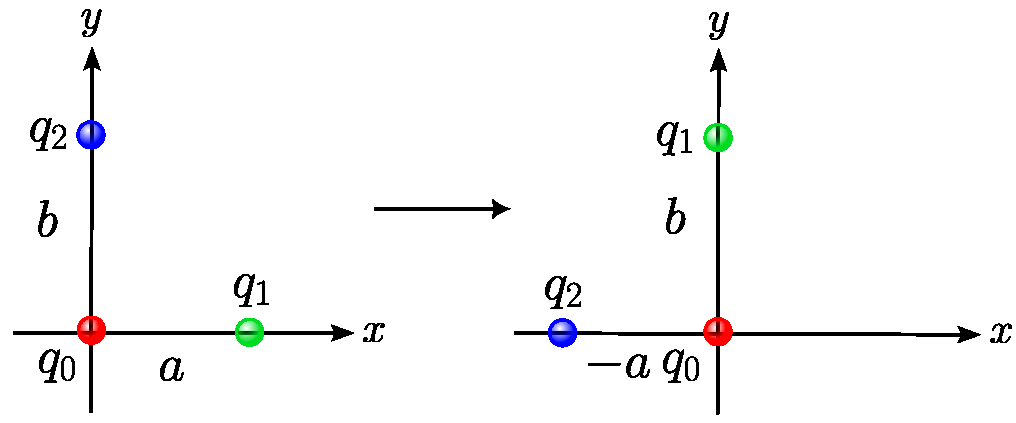
\includegraphics[scale = 0.6]{Figuras/Ej-Principio-Superposicion.pdf}
    \caption{Esquema.}
    \label{fig:Ej-Principio-Superposicion}
\end{figure}

\textbf{Solución:} Primero determinemos la fuerza neta sobre la carga $q_0$ antes del cambio de posición de las cargas.
\begin{align*}
    \vec{F}_0 &= \vec{F}_{01} + \vec{F}_{02} \\
&= k \frac{q_0q_1}{|\vec{x}_0 - \vec{x}_1|^3} (\vec{x}_0- \vec{x}_1) + k \frac{q_0q_2}{|\vec{x}_0 - \vec{x}_2|^3} (\vec{x}_0- \vec{x}_2) \\
&= k \frac{q_0q_1}{a^3} (-a \hat{\imath}) + k \frac{q_0q_2}{b^3} (-b \hat{\jmath}).
\end{align*}

Multiplicando por $\hat{\imath}$ y $\hat{\jmath}$, se obtienen las componentes (dato conocido):
\begin{align*}
    F_x &= - k \frac{q_0q_1}{a^2} \Rightarrow  q_1 = - \frac{F_x a^2}{k q_0}, \\
F_y &= - k \frac{q_0q_2}{b^2} \Rightarrow  q_2 = - \frac{F_y b^2}{k q_0}.
\end{align*}

Luego, cuando se cambia de posición las cargas, la nueva fuerza neta sobre la carga $q_0$ está dada por:
\begin{align*}
    \vec{F}_0 \,' &= \vec{F}_{01}\,' + \vec{F}_{02}\,' \\
&= k \frac{q_0q_1}{|\vec{x}_0 - \vec{x}_1\,'|^3} (\vec{x}_0- \vec{x}_1\,') + k \frac{q_0q_2}{|\vec{x}_0 - \vec{x}_2\,'|^3} (\vec{x}_0- \vec{x}_2\,') \\
&= k \frac{q_0q_1}{b^3} (-b \hat{\jmath}) + k \frac{q_0q_2}{a^3} (a \hat{\imath}).
\end{align*}

Reemplazando los valores de $q_1$ y $q_2$ en función de $F_x$ y $F_y$ encontrados.
$$\vec{F}_0\,' = - \frac{b^2}{a^2}F_y \hat{\imath} + \frac{a^2}{b^2} F_x \hat{\jmath}.$$

Por lo tanto,
$$F_x' = - \frac{b^2}{a^2}F_y ~~\mbox{y}~~ F_y' = \frac{a^2}{b^2} F_x.$$

\end{ejemplo}

\section{Ley de Coulomb para distribuciones continuas de carga}

Hemos visto que la carga eléctrica está cuantizada, pero desde el punto de vista macroscópico, puede considerarse que en los materiales las cargas pueden formar un continuo, pudiendo aplicarse en su análisis el Cálculo Diferencial.


Para aplicar la Ley de Coulomb a situaciones en que aparezcan estos materiales, se los subdivide formando elementos de carga y se aplica el principio de superposición, reemplazando la suma vectorial por una integral vectorial. Así la fuerza neta sobre una carga puntual es
$$\vec{F}_{neta} = \int d \vec{F}.$$

Por ejemplo, una carga puntual $q$ en presencia de una distribución continua de carga, donde $dq'$ es un elemento de carga de la distribución, la fuerza $d\Vec{F}$ que experimenta $q$ debido a $dq'$ es

\begin{figure}[H]
    \centering
    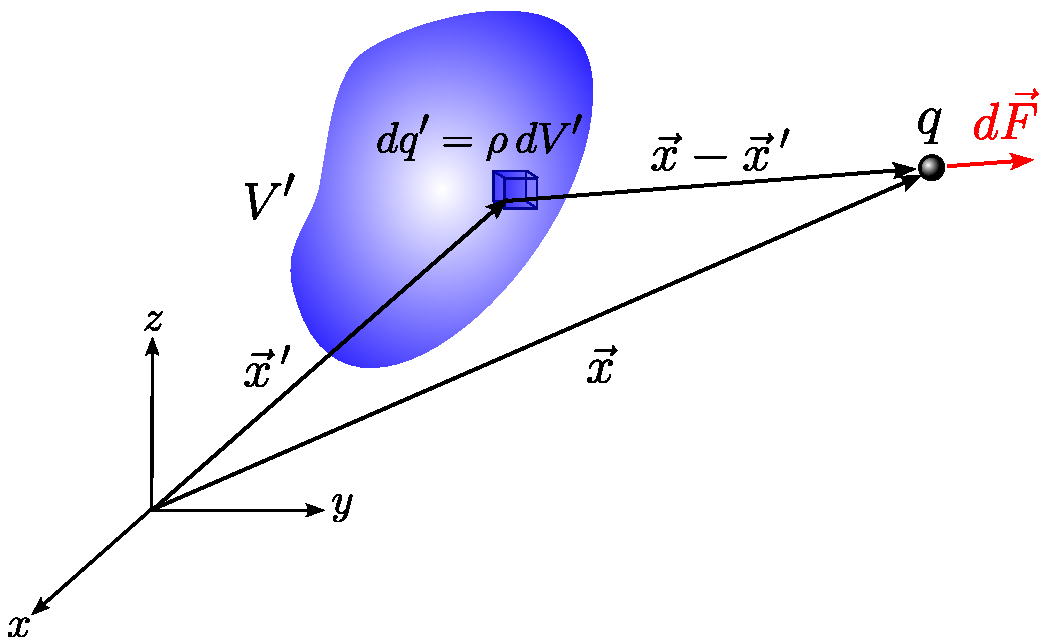
\includegraphics[scale = 0.6]{Figuras/Distribucion-Cargas-Fuerza.pdf}
    \caption{Distribución de carga.}
    \label{fig:Distribu-Carga}
\end{figure}

\begin{shaded}
   \begin{equation*}
d\vec{F} = \frac{1}{4\pi \varepsilon_0} \frac{q \,dq'}{|\vec{x} - \vec{x}\,'|^3} (\vec{x}- \vec{x}\,'),
\end{equation*} 
\end{shaded}

donde $\vec{x}$ es el vector posición de la carga $q$ (constante) y $\vec{x}\,'$ es el vector posición del elemento de carga $dq'$ (no constante).

Para el cálculo de la fuerza debemos integrar, pero necesitamos conocer la forma geométrica del cuerpo y la manera en que varía la \textbf{densidad de carga} en todos sus puntos.

En la práctica es conveniente describir la distribución de carga en función de \textit{densidades de carga}, pues la carga puede estar distribuida en una línea, superficie o volumen.

\begin{itemize}
\item[i)] \textbf{Densidad volumétrica de carga:}
\begin{equation*}
\rho = \frac{dq}{dV} ~ \left[\frac{C}{m^3} \right] \rightarrow dq' = \rho \, dV' ~\rightarrow~ d \vec{F} = k \frac{q \rho \,dV'}{|\vec{x} - \vec{x}\,'|^3} (\vec{x} - \vec{x}\,')
\end{equation*}

\item[ii)] \textbf{Densidad superficial de carga:}
\begin{equation*}
\sigma = \frac{dq}{dS} ~ \left[\frac{C}{m^2} \right] \rightarrow dq' = \sigma \, dS' \rightarrow d \vec{F} = k \frac{q \sigma \, dS'}{|\vec{x} - \vec{x}\,'|^3} (\vec{x} - \vec{x}\,')
\end{equation*}


\item[iii)] \textbf{Densidad lineal de carga:} 
\begin{equation*}
\lambda = \frac{dq}{dl} ~ \left[\frac{C}{m} \right] \rightarrow dq' = \lambda \, dl' \rightarrow d \vec{F} = k \frac{q \lambda \,dl'}{|\vec{x} - \vec{x}\,'|^3} (\vec{x} - \vec{x}\,')
\end{equation*}

\end{itemize}

En el caso de que, por ejemplo, $\rho$ sea uniforme:
\begin{equation*}
\rho = \frac{Q}{V},
\end{equation*}

donde $Q$ es la carga total y $V$ el volumen total de la distribución.

\textbf{Aclaración:} La forma en como se escribieron las densidades de carga puede resultar un poco confusa debido a que NO se trata de una derivada convencional, ésto es, $\rho$ no se obtiene al tomar $q$ como función del volumen y  derivar con respecto a $V$. Por ello, es mejor definir $\rho$ como la siguiente relación entre cantidades infinitesimales: $dq = \rho \,dV$ tal que al integrar se obtenga la carga total del sistema
$$Q = \iiint_V \rho \,dV.$$

Similarmente, para una distribución superficial y una lineal de carga:
$$Q = \iint_S \sigma\,dS \quad \text{o} \quad Q = \int_{L} \lambda \,dl.$$

\textbf{Observación:} Si las densidades de cargas $\lambda$, $\sigma$ y $\rho$ son constantes, se dice que se tiene una distribución de carga \textcolor{red}{uniforme}; pero si dependen de las coordenadas ($\rho(\vec{x}\,')$), obviamente se trata de una distribución de carga \textcolor{red}{no uniforme}.

El signo de la carga está incluido en ellas, por ejemplo,
\begin{equation*}
\lambda = -5 \times 10^{-6} ~ \left[ \frac{C}{m} \right].
\end{equation*}

\begin{ejemplo}
    Una carga eléctrica positiva $q$ está distribuida uniformente con densidad de carga $\lambda $ a lo largo de una línea de longitud $L$, que yace sobre el eje $y$ entre $y=-L$ e $y=L$. Encuentre la fuerza eléctrica que actúa sobre una carga $Q$ situada sobre el eje $x$ a una distancia $x$ del origen.

\begin{figure}[H]
    \centering
    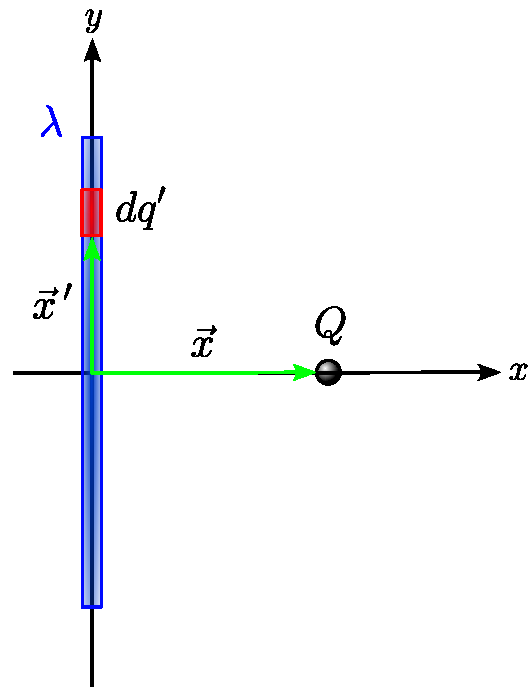
\includegraphics[scale = 0.6]{Figuras/Ej-Distribucion-Carga-1.pdf}
    \caption{Esquema de la situación física.}
    \label{fig:Ej-Distri-Carga-1}
\end{figure}

\textbf{Solución:} Usando coordenadas cartesianas, se tiene que
$$dq' = \lambda \,dy', \quad \Vec{x} = x \, \hat{\imath}, \quad \Vec{x}\,' = y' \,\hat{\jmath},$$

con $-L \leq y' \leq L$.

Por Coulomb, el diferencial de fuerza sobre $Q$ está dado por
\begin{align*}
    d\Vec{F} &= \frac{1}{4\pi \varepsilon_0}  \frac{Q \,dq'}{|\Vec{x} - \Vec{x}\,'|^3}(\Vec{x} - \Vec{x}\,') \\
    &= \frac{Q}{4\pi \varepsilon_0}  \frac{\lambda \,dy'}{|x \, \hat{\imath} - y' \,\hat{\jmath}|^3} (x \, \hat{\imath} - y' \,\hat{\jmath}) \\
    &= \frac{Q}{4\pi \varepsilon_0}  \frac{\lambda \,dy'}{(\sqrt{x^2 + y'\,^2})^3} (x \, \hat{\imath} - y' \,\hat{\jmath}).
\end{align*}

Integrando a ambos lados, la fuerza que actúa sobre $Q$ es
\begin{align*}
    \Vec{F} &= \frac{Q \lambda}{4\pi \varepsilon_0} \int_{-L}^L \frac{x \,\hat{\imath} - y' \,\hat{\jmath}}{(\sqrt{x^2 + y'\,^2})^3}  \,dy' \\
    &= \frac{Q \lambda}{4\pi \varepsilon_0} \left(x \int_{-L}^L \frac{1}{(\sqrt{x^2 + y'\,^2})^3} \,dy' \hat{\imath} + \int_{-L}^{L} \frac{y'}{(\sqrt{x^2+y'\,^2})^3} \,dy' \hat{\jmath} \right).  
\end{align*}

Usando las integrales del apéndice \ref{Integrales-Utiles}, en específico,

\begin{equation*}
\int \frac{1}{(\sqrt{x^2+y'\,^2})^3} \,dy' = \frac{y'}{x^2 \sqrt{x^2+y'\,^2}} + C \quad \text{y} \quad \int \frac{y'}{(\sqrt{x^2+y'\,^2})^3} \,dy' = - \frac{1}{\sqrt{x^2+y'\,^2}} +C,
\end{equation*}

tenemos que 
\begin{align*}
    \Vec{F} &= \frac{Q \lambda}{4\pi \varepsilon_0} \left[ x \frac{y'}{x^2 \sqrt{x^2+y'\,^2}} \hat{\imath} - \frac{1}{\sqrt{x^2+y'\,^2}} \hat{\jmath} \right]_{-L}^{L} \\
    &= \frac{Q \lambda}{4\pi \varepsilon_0} \frac{2L}{x \sqrt{x^2+L^2}} \hat{\imath}.
\end{align*}
\end{ejemplo}

\begin{ejemplo}
    Considere una distribución de carga lineal con forma de semi-circunferencia de radio $R$ y densidad de carga $\lambda$. Determine y calcule la fuerza que esta distribución ejerce sobre una carga puntual $q_0$ ubicada en el centro de curvatura.

\begin{figure}[H]
    \centering
    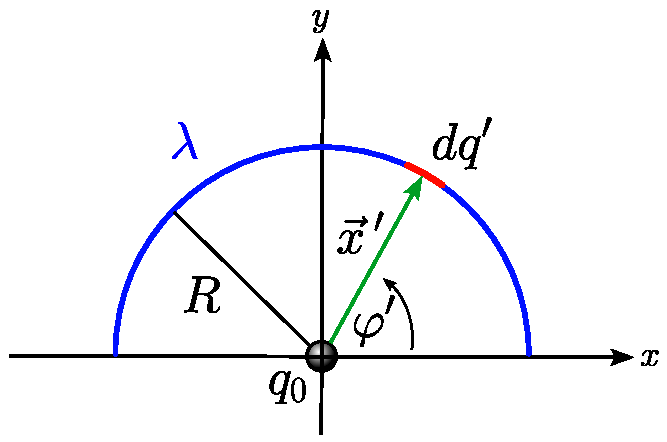
\includegraphics[scale = 0.6]{Figuras/Ej-Distribucion-Carga-2.pdf}
    \caption{Esquema de la situación física.}
    \label{fig:Ej-Distri-Carga-2}
\end{figure}


\textbf{Solución:} Usando coordenadas polares (cilíndricas con $z = 0$), se tiene que
$$dq' = \lambda R \,d\varphi', \quad \Vec{x} = \Vec{0}, \quad \Vec{x}\,' = R \,\hat{\rho} = R (\cos \varphi ' \,\hat{\imath} + \sin \varphi ' \,\hat{\jmath}),$$

con $0 \leq \varphi ' \leq \pi$.

Por Coulomb, el diferencial de fuerza sobre $q_0$ está dado por
\begin{align*}
    d\Vec{F} &= \frac{1}{4\pi \varepsilon_0}  \frac{q_0 \,dq'}{|\Vec{x} - \Vec{x}\,'|^3}(\Vec{x} - \Vec{x}\,) \\
    &= \frac{q_0}{4\pi \varepsilon_0}  \frac{\lambda R \,d\varphi'}{|\Vec{0} - R \hat{\rho}|^3} (\Vec{0} - R \,\hat{\rho}) \\
    &=- \frac{q_0}{4\pi \varepsilon_0}  \frac{\lambda R^2 \,d \varphi'}{R^3} \,\hat{\rho} \\
    &= - \frac{q_0}{4\pi \varepsilon_0}  \frac{\lambda \,d \varphi'}{R} \,\hat{\rho}.
\end{align*}

Integrando a ambos lados, la fuerza que actúa sobre $q_0$ es
\begin{align*}
\Vec{F} &=   - \frac{1}{4\pi \varepsilon_0} \frac{q_0 \lambda}{R}  \int_0^{2\pi}  \,\hat{\rho} \,d\varphi' \\
&= - \frac{1}{4\pi \varepsilon_0} \frac{q_0 \lambda}{R}  \int_0^{2\pi} \cos \varphi ' \,\hat{\imath} + \sin \varphi  '\,\hat{\jmath} \,d\varphi' \\
&= - \frac{1}{4\pi \varepsilon_0} \frac{q_0 \lambda}{R}  \left[\sin \varphi' \, \hat{\imath} - \cos \varphi\,' \,\hat{\jmath} \right]_0^{\pi} \\
&= - \frac{1}{2\pi \varepsilon_0} \frac{q_0 \lambda}{R} \, \hat{\jmath}.
\end{align*}
\end{ejemplo}

\textbf{Observación:} Note que en el primer ejemplo los vectores unitarios salieron de la integral a excepción del segundo ejemplo. Ésto es debido a que los vectores unitarios cartesianos son constantes y los cilíndricos no lo son, por ejemplo, $\hat{\rho}$ es una función de $\varphi$.

\begin{ejemplo}
    Determine la fuerza que una esfera de radio $R$, carga $Q$ y densidad de carga $\rho = cte$, ejerce sobre una carga puntual $q_0$ colocada afuera de ella.
    
\begin{figure}[H]
    \centering
    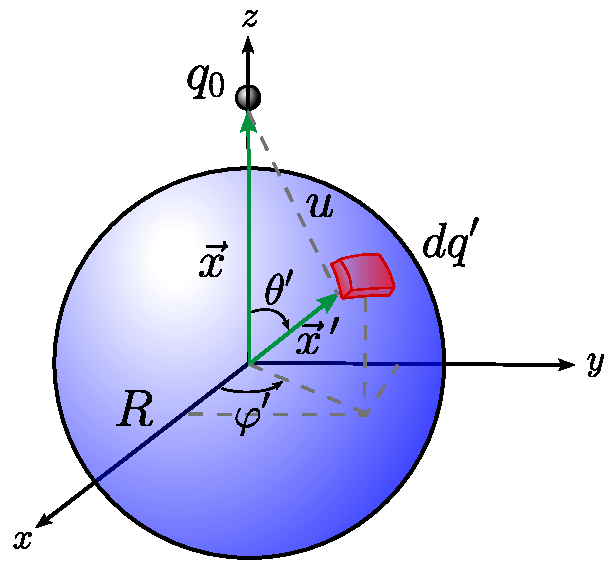
\includegraphics[scale = 0.65]{Figuras/Ej-Distribucion-Carga-3.pdf}
    \caption{Esquema de la situación física.}
    \label{fig:Ej-Distri-Carga-3}
\end{figure}

\textbf{Solución:} Consideremos una esfera maciza cargada uniformemente de radio $R$. Si nos movemos en una circunferencia de radio $r >R$ con el mismo centro que la esfera, observaremos la misma distribución y la fuerza electrostática tendrá la misma intensidad. Por lo tanto, situaremos nuestro sistema de referencia en el centro de ella y sin perder generalidad calcularemos la fuerza que ejerce la esfera sobre una carga puntual $q_0$ ubicada en el eje $z$, ver figura \ref{fig:Ej-Distri-Carga-3}.

Usando coordenadas esféricas, se tiene que
\begin{align*}
    dq' &= \rho \, dV' = \rho r'\,^2 \sin \theta' \,d \varphi' \,d\theta' \,dr', \\
    \Vec{x} \,' &= r' \,\hat{r} = r' (\cos \varphi ' \sin \theta' \,\hat{\imath} + \sin \varphi' \sin \theta' \,\hat{\jmath} + \cos \theta' \,\hat{k}),\\
    \Vec{x} &= z \,\hat{k},
\end{align*}

con $0 \leq r' \leq R$, $0 \leq \theta' \leq \pi$, $0 \leq \varphi' \leq 2\pi$ y $z\geq R$.

Por Coulomb, el diferencial de fuerza sobre $q_0$ está dado por
\begin{align*}
    d\Vec{F}&= \frac{1}{4\pi\varepsilon_0} \frac{q_0 \,dq'}{|\Vec{x} - \Vec{x}\,'|^3} (\Vec{x} - \Vec{x}\,') \\
    &= \frac{q_0 \rho}{4\pi \varepsilon_0} \frac{r'\,^2 \sin \theta' \,d \varphi' \,d\theta' \,dr' }{\left(\sqrt{z^2 + r'\,^2 - 2zr' \cos \theta'} \right)^3} (z\,\hat{k} - r' \,\hat{r}).
\end{align*}

Integrando a ambos lados, la fuerza que actúa sobre $q_0$ es
\begin{align*}
    \Vec{F} &= \frac{q_0 \rho}{4\pi \varepsilon_0} \int_0^R \int_0^{\pi} \int_0^{2\pi} \frac{r'\,^2 \sin \theta'  }{\left(\sqrt{z^2 + r'\,^2 - 2zr' \cos \theta'} \right)^3} (z\,\hat{k} - r' \,\hat{r}) \,d \varphi' \,d\theta' \,dr' \\
    &= \frac{q_0 \rho}{4\pi \varepsilon_0} \int_0^R \int_0^{\pi}  \frac{r'\,^2 \sin \theta'  }{\left(\sqrt{z^2 + r'\,^2 - 2zr' \cos \theta'} \right)^3} \left(\int_0^{2\pi} z\,\hat{k} - r' \,\hat{r} \,d \varphi' \right)\,d\theta' \,dr'.
\end{align*}

Resolvamos,
\begin{align*}
    \int_0^{2\pi} z \, \hat{k} - r' \,\hat{r}  \,d\varphi' &= \int_0^{2\pi} z \,\hat{k} - r'(\cos\varphi' \sin\theta' \, \hat{\imath} + \sin\varphi' \sin\theta' \, \hat{\jmath} + \cos\theta' \, \hat{k}) \,d\varphi' \\
    &= 2\pi (z-r'\cos\theta') \, \hat{k}.
\end{align*}

Luego,
$$\vec{F} =  \frac{ q_0 \rho}{2 \varepsilon_0} \, \hat{k} \int_0^R \int_0^{\pi} \frac{r'\,^2 \sin \theta' (z-r' \cos \theta')}{\left( \sqrt{z^2 + r'\,^2 -2zr' \cos \theta'} \right)^3} \,d\theta' \,dr'.$$

Sea $u > 0$ tal que
\begin{align*}
     u = \sqrt{z^2 + r'\,^2 - 2zr' \cos\theta'} & \Rightarrow  u^2 = z^2 + r'\,^2 - 2zr' \cos\theta' \\
     &\Rightarrow d(u^2) = \frac{d}{d \theta'} [z^2 + r'\,^2 - 2zr' \cos\theta' ] \,d\theta' \\
 & \Rightarrow  d(u^2) = 2zr' \sin \theta'\, d\theta' \\
 & \Rightarrow  u\,du = z r' \sin \theta'\, d\theta'.
\end{align*}

Usando la sustitución (altamente no trivial),
$$\cos \theta' = \frac{z^2 + r'\,^2 - u^2}{2zr'} \Rightarrow \sin \theta'\, d\theta' = \frac{u\,du}{zr'}.$$

Luego, los nuevos límites de integración son:
\begin{align*}
    \pi &\longrightarrow -2zr' = z^2+r'\,^2 -u^2 \Rightarrow  u = z + r', \\
    0 &\longrightarrow u^2 = (z-r')^2 ~\Leftrightarrow~ u = |z-r'| ~\Rightarrow ~ u = z - r'\quad (z \geq r',~ 0 \leq r' \leq R)
\end{align*}

Entonces, 
\begin{align*}
    \Vec{F} &= \frac{ q_0 \rho}{2 \varepsilon_0} \, \hat{k}  \int_0^R \left(\int_{z-r'}^{z+r'} \frac{r'\,^2}{u^3} \left(z- r' \frac{z^2 + r'\,^2 - u^2}{2z r'} \right)  \frac{u \,du}{zr'} \right) \,dr' \\
    &= \frac{ q_0 \rho}{2 \varepsilon_0} \, \hat{k}  \int_0^R \left(\int_{z-r'}^{z+r'} \frac{r'}{z u^2} \left( \frac{z^2 - r'\,^2 + u^2}{2z}  \right) \,du \right) \,dr' \\
    &= \frac{ q_0 \rho}{2 \varepsilon_0} \, \hat{k}  \int_0^R \frac{r'}{2z^2}\left(\int_{z-r'}^{z+r'}  \frac{z^2 - r'\,^2 + u^2}{u^2}  \,du \right) \,dr' \\
    &=  \frac{ q_0 \rho}{2 \varepsilon_0} \, \hat{k}  \int_0^R \frac{r'}{2z^2}\left[ u + \frac{r'\,^2 -z^2}{u} \right]_{z-r'}^{z+r'} \,dr' \\
    &= \frac{ q_0 \rho}{2 \varepsilon_0} \, \hat{k}  \int_0^R \frac{2 r'\,^2}{z^2} \,dr' \\
    &= \frac{ q_0 \rho}{2 \varepsilon_0} \, \hat{k}  \left[ \frac{2}{3z^2} r'\,^3 \right]_0^R \\
    &= \frac{q_0 \rho}{3 \varepsilon_0} \frac{R^3}{z^2} \hat{k} \\
    &= \frac{1}{4\pi \varepsilon_0} \frac{q_0 Q}{z^2} \,\hat{k},
\end{align*}

donde $\frac{4}{3} \pi R^3 \rho = Q$ con $Q$ la carga total de la esfera.
\end{ejemplo}

 \section{Campo eléctrico}

\textit{¿Cómo es posible que una carga eléctrica ejerza una fuerza sobre otra carga sin que no haya nada entremedio?}

En un principio se pensaba que las cargas ejercían una “acción a distancia”. La interpretación actual, desde \textit{Faraday }(1836), es que una carga eléctrica modifica el medio que la rodea y a la propiedad que adquiere se le llama \textbf{Campo Eléctrico} y es este campo el que actúa sobre las cargas que llegan o se encuentran en él.

Para averiguar si en un punto de un recinto existe un campo eléctrico, se coloca allí una carga de prueba $q$, supuesta positiva y pequeña con el fin de que no altere las propiedades del medio, y si dicha carga de prueba experimenta una fuerza es porque ahí existe un campo eléctrico.

Si se saca la carga de prueba, el campo sigue existiendo. Así, \textcolor{red}{el campo eléctrico es el intermediario entre las cargas que interactúan.}

Se define la \textbf{intensidad de campo eléctrico} $\vec{E}$ en un punto ($\vec{x}$) a la fuerza eléctrica en cada unidad de carga que experimenta una carga en ese punto. Se define operacionalmente como:
$$\boxed{\vec{E}(\vec{x}) := \lim_{q \to 0} \frac{\vec{F}}{q}}$$

Note que el proceso $\lim\limits_{q \to 0}$ es necesario dado que el uso de una carga $q$ de forma y magnitud arbitraria en general (mediante la interacción coulombiana) modificará la distribución de cargas original. Si la carga $q$ es cada vez más pequeña en extensión y magnitud, entonces ésta modificará cada vez menos la distribución de carga original.

Si se conoce el campo eléctrico (en el vacío), entonces la fuerza eléctrica que experimenta una carga puntual $q$ es
$$\boxed{\vec{F} = q \vec{E}(\vec{x})}$$

Supongamos que tenemos una carga $q'$ y una carga puntual $q$, por la ley de Coulomb, tenemos que
$$\vec{F} = \frac{1}{4\pi \varepsilon_0} \frac{q q'}{|\vec{x} - \vec{x}\,'|^3} (\vec{x} - \vec{x}\,').$$

Entonces, por la definición de campo eléctrico, podemos escribir
\begin{equation*}
\vec{E}(\vec{x}) = \lim_{q \to 0} \frac{\vec{F}}{q} = \frac{1}{4\pi \varepsilon_0} \frac{ q'}{|\vec{x} - \vec{x}\,'|^3} (\vec{x} - \vec{x}\,').
\end{equation*}

En general, si consideramos $q$ como un punto de campo $\vec{x}$. El \textbf{campo eléctrico} generado por $q'$ en $\vec{x}$, está dado por
\begin{shaded}
$$\vec{E}(\vec{x}) = \frac{1}{4 \pi \varepsilon_0} \frac{ q'}{|\vec{x} - \vec{x}\,'|^3} (\vec{x} - \vec{x}\,').$$
\end{shaded}

El \textbf{principio de superposición} también es aplicable al campo eléctrico. Dado un conjunto de cargas puntuales $q_1,q_2, q_3, \dots, q_n$, con vectores posición $\vec{x}_1, \vec{x}_2, \vec{x}_3, \dots , \vec{x}_n$, entonces el campo eléctrico $\vec{E}$ en un punto situado en $\vec{x}$ causado por las cargas, será
\begin{shaded}
$$\vec{E}(\vec{x}) = \frac{1}{4\pi\varepsilon_0} \sum_{i=1}^n q_i \frac{\vec{x} - \vec{x}_i}{|\vec{x} - \vec{x}_i|^3}.$$
\end{shaded}

\subsection{Campo eléctrico para distribuciones continuas}

En este caso, al igual que para la ley de Coulomb, el vector unitario, $(\vec{x} - \vec{x}\,')/|\vec{x} - \vec{x}\,'|$, tiene dirección variable, que llega al punto donde queremos calcular el campo eléctrico dado por el vector $\vec{x}$ desde el elemento de carga $dq'$.

\begin{figure}[H]
    \centering
    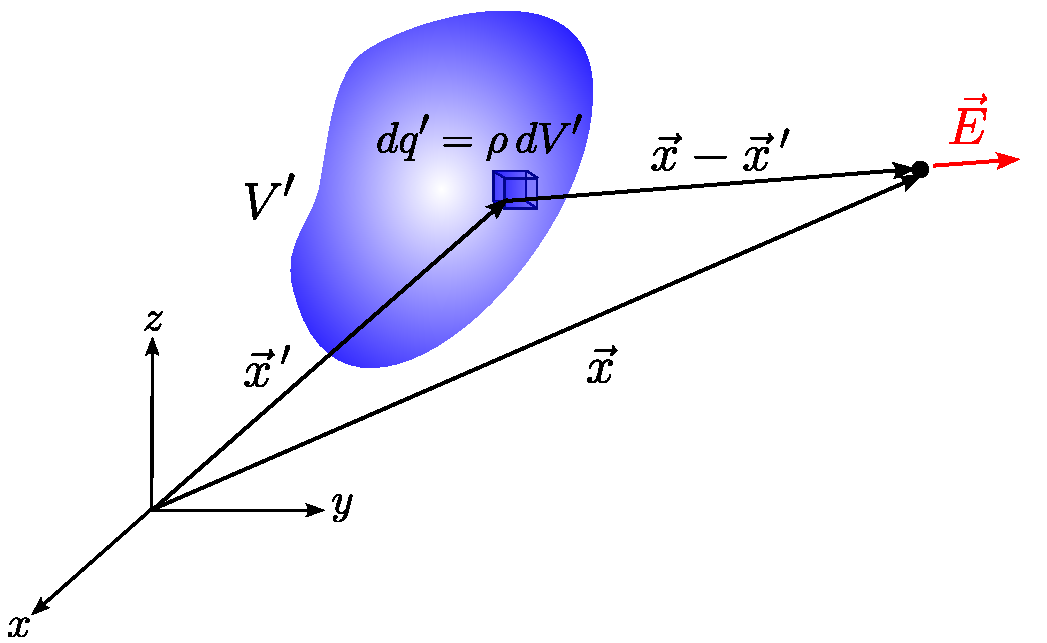
\includegraphics[scale = 0.6]{Figuras/Distribucion-Cargas-E.pdf}
    \caption{Distribución de carga.}
    \label{fig:Distribu-Carga2}
\end{figure}

\begin{equation*}
d\vec{E}(\vec{x}) = \frac{1}{4\pi \varepsilon_0} \frac{dq'}{|\vec{x} - \vec{x}\;'|^3} (\vec{x} - \vec{x}\;').
\end{equation*}

Si queremos calcular el campo eléctrico neto en $\vec{x}$, integramos ambos lados.
\begin{shaded}
    $$\vec{E}(\vec{x}) = \frac{1}{4\pi \varepsilon_0} \int \frac{dq'}{|\vec{x} - \vec{x}\;'|^3} (\vec{x} - \vec{x}\;').$$
\end{shaded}

En que, según sea el caso,
\begin{equation*}
dq = \rho \,dV = \sigma \,dS = \lambda \,dl.
\end{equation*}

\begin{ejemplo}
    Suponga que se tiene un alambre infinito sobre el eje $z$ y con densidad de carga uniforme igual a $\lambda$. Calcule el campo electrostático a una distancia $R$ del alambre.

\begin{figure}[H]
    \centering
    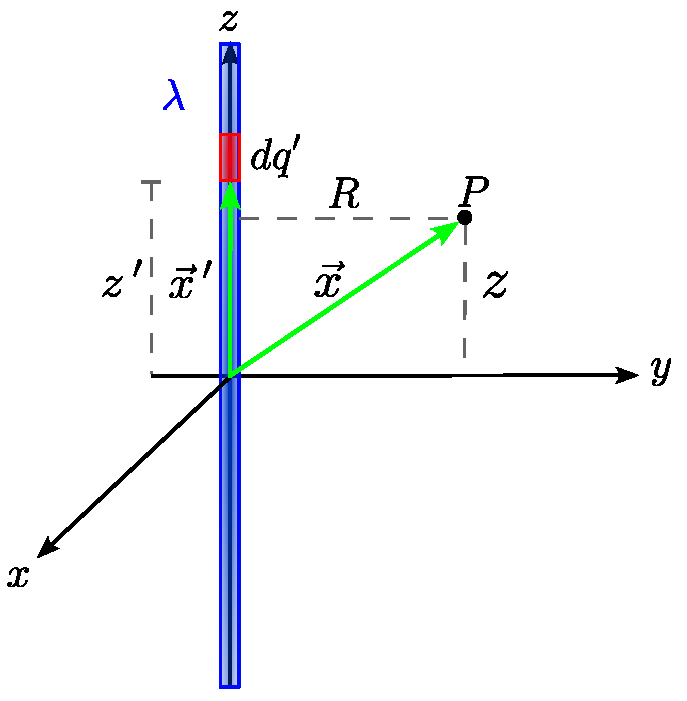
\includegraphics[scale = 0.6]{Figuras/Ej-E-Alambre-Infinito.pdf}
    \caption{Esquema de la situación física.}
    \label{fig:Ej-E-Alambre-Infinito}
\end{figure}

\textbf{Solución:} Considerando un punto $P$ cualquiera en el espacio, éste posee como vector posición:
$$\Vec{x} = R \,\hat{\rho} + z \, \hat{k}.$$

Usando coordenadas cilíndricas, se tiene que
$$dq' = \lambda \,dz', \quad \Vec{x}\,' = z' \,\hat{k},$$

con $- \infty < z' < \infty$.

Luego, el diferencial de campo eléctrico en el punto $P$ está dado por
\begin{align*}
    d \vec{E}(\vec{x}) &= \frac{1}{4\pi \varepsilon_0} \frac{dq'}{|\vec{x} - \vec{x}\,'|^3} (\vec{x} - \vec{x}\,')  \\
&= \frac{1}{4\pi \varepsilon_0} \frac{\lambda \,dz'}{|(R \,\hat{\rho} + z\, \hat{k}) - z' \,\hat{k}|^3} ((R \,\hat{\rho} + z \,\hat{k}) -z'\,\hat{k}) \\
&= \frac{\lambda}{4\pi \varepsilon_0} \frac{R \,\hat{\rho} + (z-z')\, \hat{k}}{(\sqrt{R^2 + (z-z')^2})^3} \,dz'.
\end{align*}

Integrando a ambos lados, el campo eléctrico es 
\begin{align*}
    \Vec{E}(\Vec{x}) &= \frac{\lambda}{4\pi \varepsilon_0} \int_{-\infty}^{\infty} \frac{R \,\hat{\rho} + (z-z')\, \hat{k}}{(\sqrt{R^2 + (z-z')^2})^3} \,dz' \\
    &= \frac{\lambda}{4\pi \varepsilon_0} \left[ \int_{-\infty}^{\infty} \frac{R}{(\sqrt{R^2 + (z-z')^2})^3} \,dz' \, \hat{\rho} + \int_{-\infty}^{\infty} \frac{z-z'}{(\sqrt{R^2 + (z-z')^2})^3} \,dz'\,\hat{k}\right].
\end{align*}

Si hacemos el cambio de variable $u = z - z' \Rightarrow du = - dz'$ en la segunda integral, tenemos que
$$\int_{-\infty}^{\infty} \frac{z-z'}{(\sqrt{R^2 + (z-z')^2})^3} \,dz' = \int_{\infty}^{-\infty} \frac{u}{(\sqrt{R^2 + u^2})^3} (- du) = \int_{-\infty}^{\infty} \frac{u}{(\sqrt{R^2 + u^2})^3} \,du.$$

El integrando es una función impar en $u$, ésto es, si
$$f(u) = \frac{u}{(\sqrt{R^2 + u^2})^3} \Rightarrow f(-u) = - \frac{u}{(\sqrt{R^2 + u^2})^3} = -f(u).$$

Entonces,  la integral desde $-\infty$ a $\infty$ en $u$, se anula. Así,
$$\Vec{E}(\Vec{x}) = \frac{\lambda}{4\pi \varepsilon_0}\int_{-\infty}^{\infty} \frac{R}{(\sqrt{R^2 + (z-z')^2})^3} \,dz' \, \hat{\rho} .$$

Resolviendo la integral indefinida:
$$\int \frac{R}{(\sqrt{R^2 + (z-z')^2})^3} \,dz' = - \frac{z-z'}{R\sqrt{R^2 + (z-z')^2}} + C .$$
 
Por lo tanto, 
\begin{align*}
    \vec{E}(\vec{x}) &= \frac{ \lambda}{4\pi \varepsilon_0} \left[ - \frac{z-z'}{R\sqrt{R^2 + (z-z')^2}} \right]_{-\infty}^{\infty} \hat{\rho} \\
&=  \frac{\lambda}{4\pi \varepsilon_0} \left[ - \frac{z-z'}{ R|z-z'|\sqrt{\frac{R^2}{(z-z')^2} + 1}} \right]_{-\infty}^{\infty} \hat{\rho} \\
&= \frac{\lambda}{4\pi \varepsilon_0} \left( \frac{1}{R} + \frac{1}{R} \right) \hat{\rho}  \\
&= \frac{\lambda}{2\pi \varepsilon_0 R} \,\hat{\rho}.
\end{align*}

\end{ejemplo}

\subsubsection{Campo eléctrico (radial):}

Ahora que se ha obtenido el resultado final, generalicemos para una distancia al eje $z$ arbitraria, lo cual se logra al sustituir $R \rightarrow \rho$.
$$\vec{E}(\Vec{x}) = \frac{\lambda}{2 \pi \varepsilon_0 \rho}\, \hat{\rho}.$$

En ella se observa que el campo eléctrico tiene simetría radial cilíndrica, ésto es, no depende de la coordenada $z$, el vector unitario tiene dirección perpendicular al alambre, y también se observa que la magnitud del campo es inversamente proporcional a la primera potencia de $\rho$.

\textbf{Observación:} Que sea inversamente proporcional a $\rho$ y no a $\rho^2$ significa que el campo de una línea o alambre es más intenso que si fuera el de una carga puntual. Además, este resultado es válido si el alambre es infinito o muy largo tal que no podemos ver los extremos, pues si es finito, al acercarnos a los extremos, el campo eléctrico tendrá una componente en $z$.

\begin{figure}[H]
\centering
\resizebox{12cm}{6cm}{%
\begin{tikzpicture}
[decoration={markings, 
	mark= at position 0.7 with {\arrow[]{latex}}}
] 

% Solve rotation issue
\path[] (-2,-3) rectangle (13.5,5);

% Rotate the illustration
\begin{scope}[transform canvas={rotate=10}]

% Electric Field (arrows of back layer) 
% 3D version
   
   \foreach \j in {1.25,5.75,9.75}
{
\draw[xshift=\j cm] (0,0) ellipse(0.2 and 0.5);
    \begin{scope}[xshift=\j cm,tdplot_main_coords]

        \foreach \angle in {0,45,...,180}
{
\tdplotsetcoord{P2}{2}{\angle}{-40}
\tdplotsetcoord{P1}{0.5}{\angle}{-40}
\draw[thick,postaction={decorate}] (P1) -- (P2);

}
    \end{scope}
}



% Cylindrical shape
\draw [top color= OliveGreen,
			bottom color= OliveGreen,
			middle color=YellowGreen,
			opacity=0.92] (0,-0.5) -- ++(12,0) 
	arc(-90:90:0.2 and 0.5) -- ++(-12,0) 
	arc(90:-90:0.2 and 0.5)--cycle;

\draw[fill=cyan!10] (0,0) ellipse(0.2 and 0.5);



% Electric charge
\foreach \j in {1,3.5,7,11} 
{
	\node at (\j,0){$\textbf{+}$};
}

% Electric Field (arrows of front layer) 
% 3D version

\foreach \j in {1.25,5.75,9.75}
{
    \begin{scope}[xshift=\j cm,tdplot_main_coords]
        \foreach \angle in {180,225,...,360}
{
\tdplotsetcoord{P2}{2}{\angle}{-40}
\tdplotsetcoord{P1}{0.5}{\angle}{-40}
\draw[thick,postaction={decorate}] (P1) -- (P2);

}
    \end{scope}
}


\end{scope} % end scope of the illustration rotation

\end{tikzpicture}
}
\caption{Campo eléctrico de un alambre infinito. Recuperado de: \href{https://latexdraw.com/electric-field-of-line-charge-in-tikz/}{latexdraw.com}.}
\end{figure}

\begin{ejemplo}
     Calcule el campo electrostático en un punto arbitrario que no se encuentre en el plano generado por un plano infinito que posee una densidad de carga uniforme $\sigma$. 

\begin{figure}[H]
    \centering
    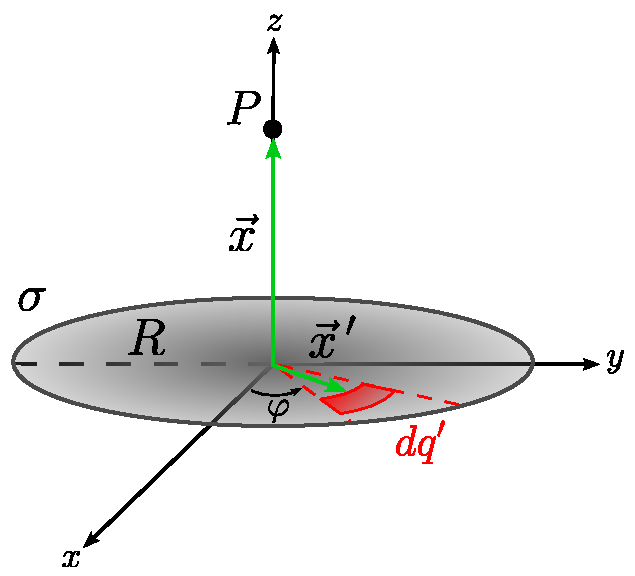
\includegraphics[scale = 0.65]{Figuras/Ej-E-Plano-Infinito.pdf}
    \caption{Esquema de la situación física.}
    \label{fig:Ej-E-Plano-Infinito}
\end{figure}

\textbf{Solución:} Si tenemos un plano infinito y tomamos un punto $P$ que no se encuentre en el plano. Podemos calcular el campo eléctrico en $P$ en el eje $z$, pues se puede tomar un vector normal al plano con dirección pasando por $P$, y un disco de centro en el origen y radio $R$ que se aplicará la condición $R \rightarrow \infty$ para tener el plano infinito, ver figura \ref{fig:Ej-E-Plano-Infinito}.

Usando coordenadas cilíndricas, se tiene que
$$dq' = \sigma \rho \, d\varphi' \,d\rho', \quad \Vec{x} = z \,\hat{k}, \quad \vec{x}\,' = \rho' \,\hat{\rho} = \rho' (\cos \varphi' \,\hat{\imath} + \sin \varphi' \, \hat{\jmath}),$$

con $0 \leq \rho' \leq R$, $0 \leq \varphi ' \leq 2\pi$.

Entonces, el diferencial de campo eléctrico en $\vec{x}$ es
\begin{align*}
    d\Vec{E}(\Vec{x}) &= \frac{1}{4\pi \varepsilon_0} \frac{dq'}{|\vec{x}  - \vec{x}\,'|^3} (\vec{x} - \vec{x}\,') \\
    &=  \frac{\sigma}{4\pi \varepsilon_0} \frac{z \,\hat{k} - \rho' \,\hat{\rho}}{\left( \sqrt{z^2 + \rho'\,^2} \right)^3}\, \rho' \,d\varphi\,' d\rho'.
\end{align*}

Integrando a ambos lados, el campo eléctrico está dado por
\begin{align*}
    \Vec{E}(\Vec{x}) &= \frac{\sigma}{4\pi \varepsilon_0} \int_0^R \int_0^{2\pi} \frac{z \,\hat{k} - \rho' \,\hat{\rho}}{\left( \sqrt{z^2 + \rho'\,^2} \right)^3} \,\rho' \,d\varphi\,' d\rho' \\
    &= \frac{\sigma}{4\pi \varepsilon_0} \int_0^R \frac{\rho'}{\left( \sqrt{z^2 + \rho'\,^2} \right)^3} \left(\int_0^{2\pi} (z \,\hat{k} - \rho' \,\hat{\rho} ) \,d\varphi\,' \right)d\rho' \\
    &= \frac{\sigma}{4\pi \varepsilon_0} \int_0^R \frac{\rho'}{\left( \sqrt{z^2 + \rho'\,^2} \right)^3} \left(\int_0^{2\pi} z \,\hat{k} \,d\varphi' - \rho' \int_0^{2\pi} \hat{\rho}  \,d\varphi\,' \right)d\rho' .
\end{align*}


Como 
$$\int_0^{2\pi} \hat{\rho} \,d\varphi' = \int_0^{2\pi} (\cos \varphi' \, \hat{\imath} + \sin \varphi'\,\hat{\jmath}) \, d\varphi' = \Vec{0},$$

se tiene que 
\begin{align*}
    \Vec{E}(\Vec{x}) &= \frac{\sigma}{4\pi \varepsilon_0} \int_0^R \frac{\rho'}{\left( \sqrt{z^2 + \rho'\,^2} \right)^3} \left(\int_0^{2\pi} z \,\hat{k} \,d\varphi'\right)d\rho' \\
    &= \frac{\sigma}{4\pi \varepsilon_0} \int_0^R \frac{\rho'}{\left( \sqrt{z^2 + \rho'\,^2} \right)^3} \, 2\pi z \, \hat{k} d\rho' \\
    &= \frac{\sigma}{2 \varepsilon_0} z \,\hat{k} \int_0^R\frac{\rho'}{\left( \sqrt{z^2 + \rho'\,^2} \right)^3} \,d\rho'.
\end{align*}

Usando la integral \eqref{A-I3} del apéndice \ref{Integrales-Utiles}, se obtiene
\begin{align*}
    \Vec{E}(\Vec{x}) &= \frac{\sigma z}{2 \varepsilon_0}  \,\hat{k} \left[ - \frac{1}{\sqrt{z^2 + \rho'\,^2}}\right]_0^R \\
    &= \frac{\sigma z}{2 \varepsilon_0}  \left(\frac{1}{|z|} - \frac{1}{\sqrt{z^2 + R^2}} \right) \,\hat{k}.
\end{align*}

Finalmente, tomamos el límite cuando $R \to \infty$.
\begin{align*}
    \lim_{R \to \infty} \Vec{E}(\Vec{x}) &= \frac{\sigma z}{2 \varepsilon_0}  \lim_{R\to \infty} \left(\frac{1}{|z|} - \frac{1}{\sqrt{z^2 + R^2}}\right) \hat{k} \\
    &= \frac{\sigma z}{2 \varepsilon_0 |z|} \,\hat{k}.  .
\end{align*}

Por lo tanto, el campo eléctrico de un plano infinito, en cualquier punto del espacio, es
\begin{equation*}
\vec{E}(\vec{x}) = \left\{ \begin{array}{c}
\scaleto{\frac{\sigma}{2 \epsilon_0}}{20pt} \, \hat{k} ~~,~~ \mbox{si} ~z>0 \\ \\
-\scaleto{\frac{\sigma}{2 \epsilon_0} }{20pt}\, \hat{k} ~,~~\mbox{si}  ~z<0
\end{array} \right.
\end{equation*}
\end{ejemplo}

\begin{ejemplo}
    Considere un cascarón esférico de radio $R$ y con densidad de carga uniforme $\sigma$. Calcule la intensidad del campo electrostático en un punto al interior del cascarón.
    
\begin{figure}[H]
    \centering
    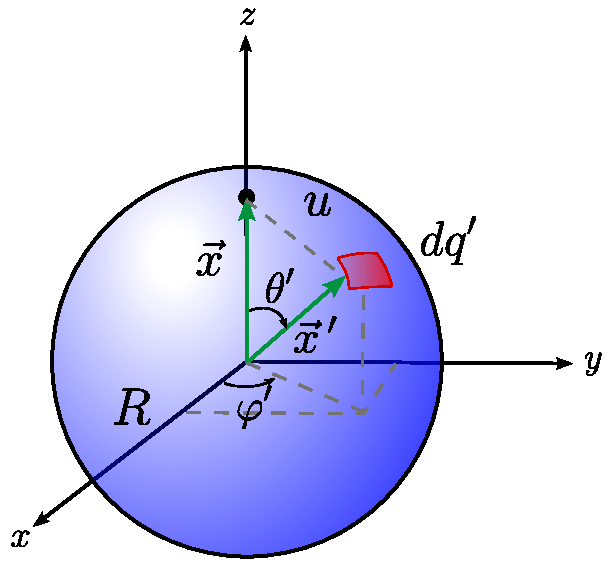
\includegraphics[scale = 0.65]{Figuras/Ej-E-Cascaron-Esferico.pdf}
    \caption{Esquema de la situación física.}
    \label{fig:Ej-E-Cascaron}
\end{figure}

\textbf{Solución:} Consideremos un cascarón esférico cargado uniformemente de radio $R$. Si nos movemos en una circunferencia de radio $r < R$ con el mismo centro que la esfera, observaremos la misma distribución y el campo eléctrico tendrá la misma intensidad. Por lo tanto, situaremos nuestro sistema de referencia en el centro de ella y sin perder generalidad calcularemos el campo electrostático en un punto situado en el eje $z$, ver figura \ref{fig:Ej-E-Cascaron}.

Usando coordenadas esféricas, se tiene que
\begin{align*}
    dq' &= \sigma R^2 \sin \theta\,d\theta'\,d\varphi', \\
    \Vec{x} &= z \, \hat{k}, \\
    \Vec{x}\,' &= R \,\hat{r} = R (\sin \theta' \cos \varphi' \, \hat{\imath} + \sin \theta' \sin\varphi' \,\hat{\jmath} + \cos \theta' \,\hat{k}),
\end{align*}

con $0 \leq \theta' \leq \pi$, $0 \leq \varphi' \leq 2\pi$ y $0 < z < R$.

Entonces, el diferencial de campo eléctrico en $\vec{x}$ es
\begin{align*}
    d\Vec{E}(\Vec{x}) &= \frac{1}{4\pi \varepsilon_0} \frac{dq'}{|\Vec{x} - \Vec{x}\,'|^3} (\Vec{x} - \Vec{x}\,') \\
    &= \frac{\sigma}{4\pi \varepsilon_0} \frac{R^2 \sin \theta'\, d\theta' \,d\varphi'}{|z\,\hat{k} - R\,\hat{r}|^3} (z\,\hat{k} - R \hat{r}) \\
    &= \frac{\sigma}{4\pi \varepsilon_0} \frac{z\,\hat{k} - R \hat{r}}{\left( \sqrt{z^2 + R^2 - 2zR \cos \theta'}\right)^3} R^2 \sin \theta' \,d\theta'\,d\varphi'.
\end{align*}

Integrando a ambos lados, el campo eléctrico está dado por
\begin{align*}
    \Vec{E}(\Vec{x}) &= \frac{\sigma R^2}{4\pi \varepsilon_0} \int_0^{\pi} \int_0^{2\pi} \frac{\sin \theta' (z\,\hat{k} - R \hat{r})}{\left( \sqrt{z^2 + R^2 - 2zR \cos \theta'}\right)^3} \,d\varphi'\,d\theta' \\
    &= \frac{\sigma R^2}{4\pi \varepsilon_0} \int_0^{\pi} \frac{\sin \theta'}{\left( \sqrt{z^2 + R^2 - 2zR \cos \theta'}\right)^3} \left( \int_0^{2\pi} (z\,\hat{k} - R \, \hat{r}) \,d\varphi'  \right)  \,d\theta'. 
\end{align*}

Resolvamos,
\begin{align*}
  \int_0^{2\pi} (z\,\hat{k} - R \, \hat{r}) \,d\varphi' &=    \int_0^{2\pi} (z\,\hat{k} - R (\sin \theta' \cos \varphi' \, \hat{\imath} + \sin \theta' \sin\varphi' \,\hat{\jmath} + \cos \theta' \,\hat{k})) \,d\varphi' \\
  &= 2\pi (z - R\cos\theta') \,\hat{k}.
\end{align*}

Luego,
$$\Vec{E}(\Vec{x}) = \frac{\sigma R^2}{2 \varepsilon_0} \,\hat{k} \int_0^{\pi} \frac{\sin \theta'(z-R \cos \theta')}{\left( \sqrt{z^2 + R^2 - 2zR \cos \theta'}\right)^3}   \,d\theta'.$$

Sea $u > 0$ tal que
\begin{align*}
     u = \sqrt{z^2 + R^2 - 2zR \cos\theta'} & \Rightarrow  u^2 = z^2 + R^2 - 2zR \cos\theta' \\
     &\Rightarrow d(u^2) = \frac{d}{d \theta'} [z^2 + R^2 - 2zR \cos\theta' ] \,d\theta' \\
 & \Rightarrow  d(u^2) = 2zR \sin \theta'\, d\theta' \\
 & \Rightarrow  u\,du = z R \sin \theta'\, d\theta'.
\end{align*}

Usando la sustitución (altamente no trivial),
$$\cos \theta' = \frac{z^2 + R^2 - u^2}{2zR} \Rightarrow \sin \theta'\, d\theta' = \frac{u\,du}{zR}.$$

Luego, los nuevos límites de integración son:
\begin{align*}
    \pi &\longrightarrow -2zR = z^2+R^2 -u^2 \Rightarrow  u = z + R, \\
    0 &\longrightarrow u^2 = (z-R)^2 ~\Leftrightarrow~ u = |z-R| ~\Rightarrow ~ u =  R - z \quad (0 < z < R).
\end{align*}

Entonces, 
\begin{align*}
    \Vec{E}(\Vec{x}) &= \frac{\sigma R^2}{2 \varepsilon_0} \,\hat{k} \int_{R-z}^{R+z} \frac{1}{u^3} \left( z - \frac{z^2+R^2-u^2}{2z}\right) \frac{u}{zR} \,du \\
    &= \frac{\sigma R^2}{2 \varepsilon_0} \,\hat{k} \int_{R-z}^{R+z} \frac{z^2 - R^2 + u^2}{2z} \cdot \frac{1}{u^2 z R} \,du \\
    &= \frac{\sigma R}{4 \varepsilon_0 z^2} \,\hat{k} \int_{R-z}^{R+z} \frac{z^2 - R^2 + u^2}{u^2}  \,du \\
    &= \frac{\sigma R}{4 \varepsilon_0 z^2} \,\hat{k} \left[u + \frac{R^2 - z^2}{u} \right]_{R-z}^{R+z} \\
    &= \frac{\sigma R}{4 \varepsilon_0 z^2} \,\hat{k} \left[2z + \frac{R^2-z^2}{R+z} - \frac{R^2-z^2}{R-z} \right] \\
    &= \Vec{0}.
\end{align*}

Para $z = 0$ (el origen) queda de ejercicio probar que también $\vec{E}(\vec{0}) = \vec{0}$.
\end{ejemplo}
 
\section{Líneas de campo eléctrico}

Las \textbf{líneas de campo eléctrico} son líneas que intentan representarlo. Convenimos en dibujarlas en la dirección y sentido del campo eléctrico, de tal manera que el campo resulta \underline{tangente} a estas líneas. En un región en que el campo es continuo no se puede dibujar todas las líneas y es necesario espaciarlas. Estas líneas no se cortan ya que el campo es único.


\begin{itemize}
\item[a)] Para una carga puntual: 

\begin{figure}[H]
        \centering
        \subfigure[]{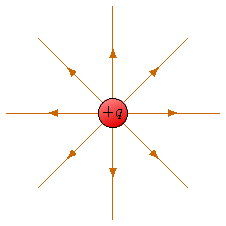
\includegraphics[width=0.36\textwidth]{Figuras/Campo-E-Carga+.pdf}} \hspace{1cm}
        \subfigure[]{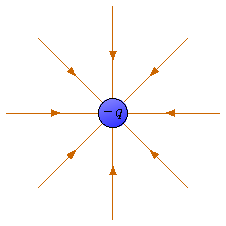
\includegraphics[width=0.36\textwidth]{Figuras/Campo-E-Carga-.pdf}} 
        \caption{Campo eléctrico de cargas puntuales positivas (a) y negativas (b). Recuperado de: \href{https://tikz.net/electric_fieldlines1/}{tikz.net}. }
        \label{fig:Campo-Cargas-Puntuales-1}
    \end{figure}

\item[b)] Para dos cargas puntuales de igual valor:

\begin{figure}[H]
        \centering
        \subfigure[]{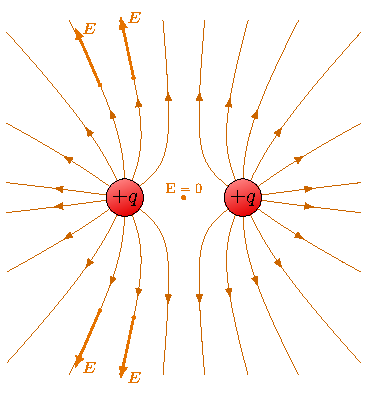
\includegraphics[width=0.36\textwidth]{Figuras/Campo-E-CargasIguales.pdf}} \hspace{1cm}
        \subfigure[]{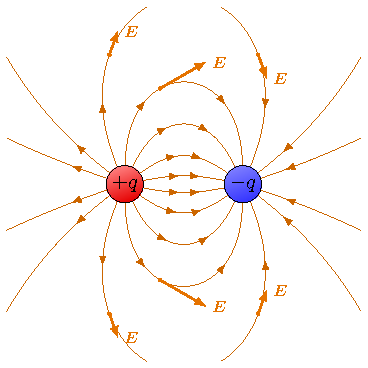
\includegraphics[width=0.36\textwidth]{Figuras/Campo-E-CargasOpuestas-.pdf}} 
        \caption{Campo eléctrico de dos cargas puntuales positivas (a) y opuestas (b). Recuperado de: \href{https://tikz.net/electric_fieldlines2/}{tikz.net}. }
        \label{fig:Campo-Cargas-Puntuales-2}
    \end{figure}

\item[c)] Para dos cargas puntuales de diferentes valores:

\begin{figure}[H]
        \centering
        \subfigure[]{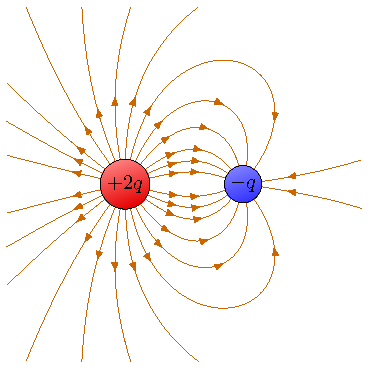
\includegraphics[width=0.36\textwidth]{Figuras/Campo-E-Cargas-MagDistintas-1.pdf}} \hspace{1cm}
        \subfigure[]{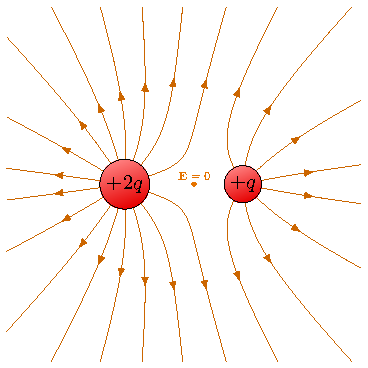
\includegraphics[width=0.36\textwidth]{Figuras/Campo-E-Cargas-MagDistintas-2.pdf}} 
        \caption{Campo eléctrico de cargas puntuales opuestas con distintos valores (a) y positivas con distintos valores (b). Recuperado de: \href{https://tikz.net/electric_fieldlines2/}{tikz.net}. }
        \label{fig:Campo-Cargas-Puntuales-3}
\end{figure}

\end{itemize}

\section{Flujo eléctrico}

Consideremos un campo vectorial que representa  al campo eléctrico generado por cargas en reposo. De ésta manera, el \textbf{flujo de campo eléctrico} queda definido por:
\begin{shaded}
    $$\Phi_E = \iint_S \Vec{E} \cdot d\Vec{S}.$$
\end{shaded}

Esta cantidad matemática mide el número de líneas que pasan a través de una superficie.

Las unidades de medida se desprenden de la definición: $[\Phi] = [\frac{N}{C} \,m^2]$.

Hay que notar que la superficie puede ser abierta o cerrada. En el caso de una \textit{superficie cerrada} el flujo se denota:
\begin{shaded}
    $$\Phi_E = \oiint_S \Vec{E} \cdot d\Vec{S}.$$
\end{shaded}

\textbf{Observación:} Si dentro de la superficie cerrada no hay ninguna carga, el número de líneas que entran en la superficie es igual al número de líneas que salen de ella. De este modo, el flujo neto será cero. 

Lo anterior se puede ver en el siguiente ejemplo.

\begin{ejemplo}
    Dado un campo eléctrico uniforme, calcule el flujo eléctrico a través de la superficie de un cubo y un cilindro tal como se indica en la figura \ref{fig:Flujo-E}.

\begin{figure}[H]
    \centering
    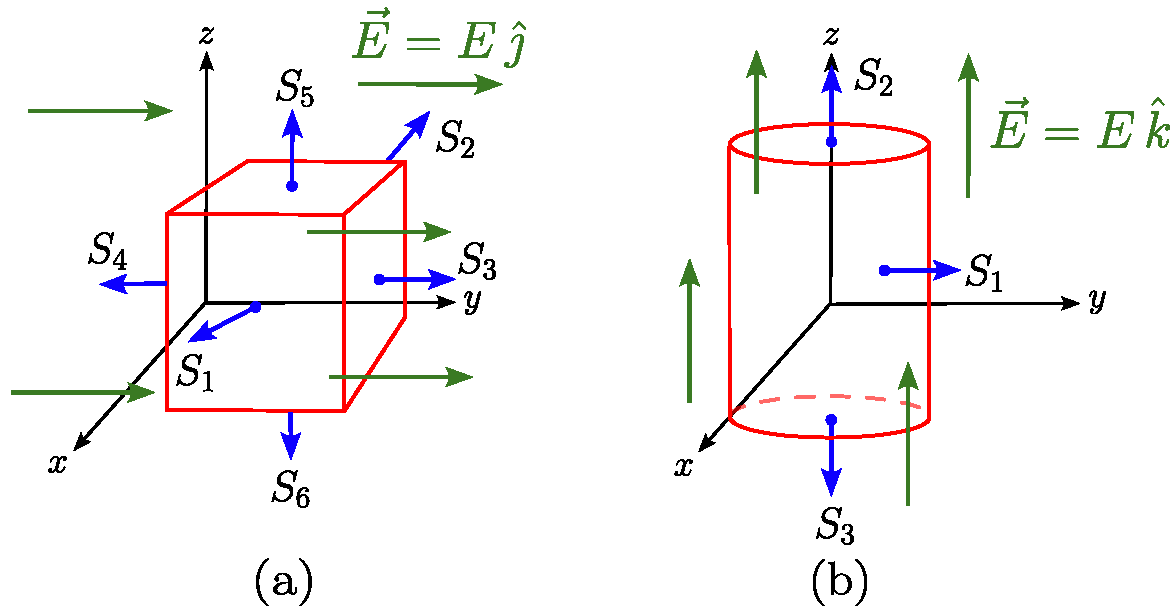
\includegraphics[scale = 0.6]{Figuras/Ej-Flujo-Electrico.pdf}
    \caption{Un cubo en presencia de un campo eléctrico uniforme en la dirección del eje $y$ (a) y un cilindro en presencia de un campo eléctrico uniforme en la dirección del eje $z$.}
    \label{fig:Flujo-E}
\end{figure}

\textbf{Solución:} Para el caso del cubo.
\begin{align*}
    \Phi_E &= \oiint_S \vec{E} \cdot d\vec{S} \\
&= \iint_{S_1} \vec{E} \cdot d\vec{S}_1 +  \iint_{S_2}\vec{E} \cdot d\vec{S}_2 + \iint_{S_3}\vec{E} \cdot d\vec{S}_3 \\
&\quad + \iint_{S_4}\vec{E} \cdot d\vec{S}_4 + \iint_{S_5}\vec{E} \cdot d\vec{S}_5 + \iint_{S_6}\vec{E} \cdot d\vec{S}_6  \\
&= \iint_{S_1} (E \hat{\jmath})\cdot(dydz \hat{\imath}) +  \iint_{S_2} (E \hat{\jmath})\cdot(-dydz \hat{\imath}) + \iint_{S_3} (E \hat{\jmath})\cdot(dxdz \hat{\jmath}) \\
&\quad + \iint_{S_4} (E \hat{\jmath})\cdot(-dxdz \hat{\jmath}) + \iint_{S_5} (E \hat{\jmath})\cdot(dxdy \hat{k}) + \iint_{S_6} (E \hat{\jmath})\cdot(-dxdy \hat{k}) \\
&= E \iint_{S_3} dxdz - E \iint_{S_4} dxdz\\
&= 0.
\end{align*}

Para el caso del cilindro:
\begin{align*}
\Phi_E &= \oiint_S \vec{E} \cdot d\vec{S} \\
&= \iint_{S_1}\vec{E} \cdot d\vec{S}_1 +  \iint_{S_2}\vec{E} \cdot d\vec{S}_2 + \iint_{S_3}\vec{E} \cdot d\vec{S}_3 \\
&= \iint_{S_1} (E \hat{k})\cdot(\rho d\varphi dz \hat{\rho}) +  \iint_{S_2} (E \hat{k})\cdot( \rho d\rho d\varphi \hat{k}) + \iint_{S_3} (E \hat{k})\cdot( -\rho d\rho d\varphi \hat{k})  \\
&= E \iint_{S_2} \rho d\rho d\varphi  - E \iint_{S_3} \rho d\rho d\varphi  = 0.
\end{align*}


\end{ejemplo}

Un caso especial es cuando el campo eléctrico es uniforme, de tal manera que puede salir fuera de la integral.
$$\Phi_E = \iint_S \vec{E} \cdot d\vec{S} = \iint_S E dS \cos \theta = E \iint_S dS \cos \theta.$$

Es más, si el campo eléctrico es \underline{perpendicular} a la superficie ($\theta = 0$), se tiene
$$\Phi_E = E \iint_S dS \cos 0 = E \iint_S dS = E A,$$

donde $A$ es el área de la superficie.

\section{Ley de Gauss} \label{Ley-Gauss}

\subsection{Forma integral de la ley de Gauss}

La \textbf{ley de Gauss} es una consecuencia de la ley de Coulomb, \footnote{La demostración matemática de la ley de Gauss se escapa de los contenidos del curso.} pero está formulada de una manera tal que permite calcular fácilmente los campos eléctricos producidos por distribuciones de carga altamente simétricas. Por ejemplo: esferas aisladas, esferas concéntricas, cilindros aislados,
cilindros concéntricos, lineas rectas, planos aislados, planos paralelos, etc.

\textbf{Enunciado:} El flujo eléctrico total que atraviesa una superficie cerrada arbitraria es igual a la carga total encerrada dividida por la permitividad eléctrica del vacío $\varepsilon_0$.
\begin{shaded}
  $$\Phi_e = \oiint_S \vec{E} \cdot d\vec{S} = \frac{q_{encerrada}}{\varepsilon_0}. $$
\end{shaded}

La superficie $S$ se llama \textbf{superficie Gaussiana} y es una superficie imaginaria (matemática) que sirve para calcular la integral de superficie $\oint_S \vec{E} \cdot d\vec{S}$. La idea es escoger una superficie conveniente con el objetivo de facilitar el cálculo de la integral, para ello es crucial saber la forma del campo eléctrico.

Esta ley puede interpretarse, en electrostática, entendiendo el flujo como una medida del número de líneas de campo que atraviesan la superficie en cuestión. Para una carga puntual es evidente que este número es constante si la carga está contenida por la superficie y es nulo si está fuera. Además, al ser la densidad de líneas proporcionales a la magnitud de la carga, resulta que este flujo es proporcional a la carga, si está encerrada, o nulo, si no lo está.

\begin{figure}[H]
    \centering
    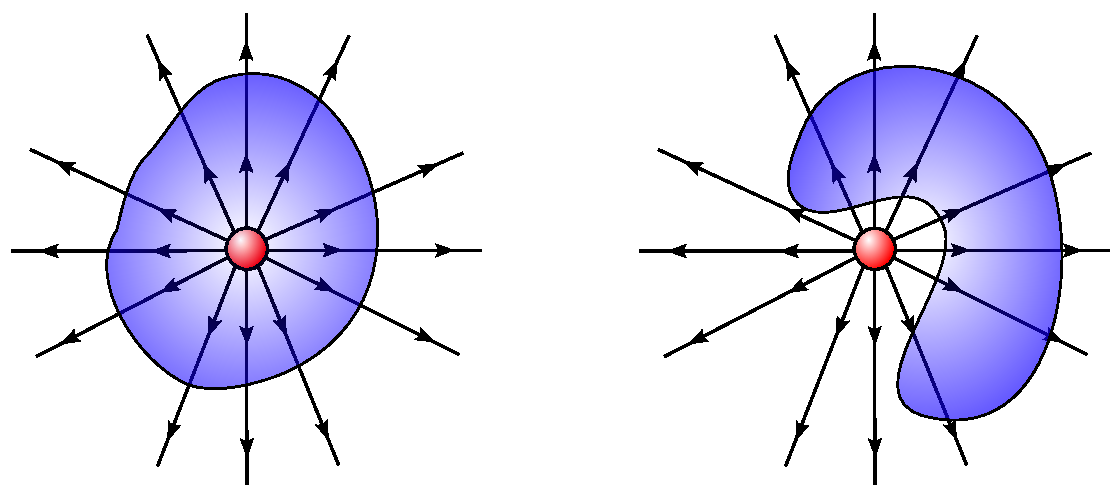
\includegraphics[scale = 0.6]{Figuras/LeyGauss.pdf}
    \caption{}
    \label{fig:Gauss-Law}
\end{figure}

Cuando tenemos una distribución de cargas, por el principio de superposición, sólo tendremos que considerar las cargas interiores, resultando la \textit{ley de Gauss}.

\begin{ejemplo}
     Una esfera de radio $R$ tiene una densidad volumétrica de carga $\rho = cte$. Determinar el campo eléctrico a) afuera de la esfera y b) adentro de ella.

\begin{figure}[H]
    \centering
    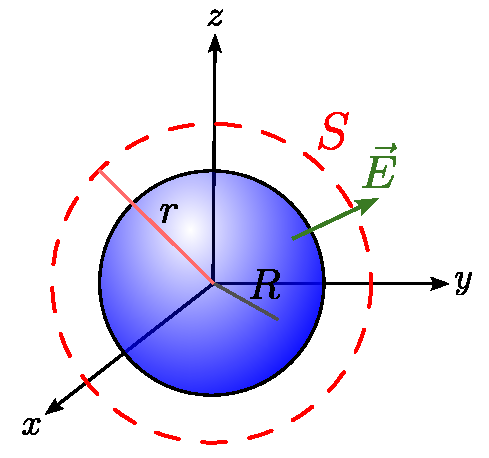
\includegraphics[scale = 0.7]{Figuras/Ej-Gauss-1.pdf}
    \caption{Superficie Gaussiana para la esfera de radio $R$ cargada uniformemente.}
    \label{fig:Ej-Gauss-1}
\end{figure}

\textbf{Solución:} El campo eléctrico de la esfera es radial, es decir, $\vec{E} = E \,\hat{r}$. Por ello, se aplicará la ley de Gauss utilizando como \textit{superficie Gaussiana} ($S$) el cascarón de una esfera centrada en el origen con radio $r$, donde el módulo del campo es constante a esa distancia.

\begin{itemize}
\item[a)] Para $r > R$, usando coordenadas esféricas, se tiene que

\begin{itemize}
\item $dq' = \rho r'\,^2 \sin \theta ' \,d\varphi'\, d\theta' dr'$ 

\item $d\vec{S} = r^2 \sin \theta \,d\varphi\, d\theta \, \hat{r}$ (diferencial de superficie de $S$).
\end{itemize}

Por la Ley de Gauss, tenemos que
\begingroup
\allowdisplaybreaks
\begin{align*}
    \oiint_S \vec{E} \cdot d\vec{S} &= \frac{q_{encerrada}}{\varepsilon_0} \\
    \int_0^{\pi} \int_0^{2\pi} (E \,\hat{r}) \cdot (r^2 \sin \theta\, d\varphi \,d\theta \,\hat{r}) &= \frac{1}{\varepsilon_0} \int_0^Q dq' \\
    \int_0^{\pi} \int_0^{2\pi} E   r^2 \sin \theta \, d\varphi \,d\theta &= \frac{1}{\varepsilon_0} \int_0^R\int_0^{\pi}\int_0^{2\pi} \rho r'\,^2  \sin \theta'\, d\varphi'\, d\theta'\, dr' \\
    2\pi E r^2 \int_0^{\pi} \sin \theta \,d\theta &= \frac{2\pi \rho}{\varepsilon_0} \int_0^R r'^2 \left( \int_0^\pi \sin \theta'\, d\theta' \right)  dr' \\ 
    4\pi r^2 E &= \frac{4}{3\varepsilon_0} \pi R^3 \rho \\
    E &= \frac{R^3 \rho}{3 \varepsilon_0 r^2}.
\end{align*}
\endgroup

Por lo tanto, 
$$\vec{E}(\vec{x}) = \frac{R^3 \rho}{3 \varepsilon_0 r^2} \,\hat{r} = \frac{1}{4\pi \varepsilon_0} \frac{Q}{r^2}\, \hat{r}, \quad r > R,$$ 

donde $Q$ es la carga total de la esfera.

\item[b)] Para $0 \leq r < R$, se tiene que la superficie Gaussiana encierra una esfera y un cascarón esférico, el campo que contribuye el cascarón es cero, por lo tanto el campo que a traviesa $S$ es radial (campo exterior de una esfera).

Usando coordenadas esféricas, se tiene que

\begin{itemize}
\item $dq' = \rho r'\,^2 \sin \theta'\, d\varphi'\, d\theta'\, dr'$ 

\item $d\vec{S} = r^2 \sin \theta\, d\varphi\, d\theta\, \hat{r}$ (diferencial de superficie de $S$).
\end{itemize}

Por la Ley de Gauss, tenemos que
\begin{align*}
    \oiint_S \vec{E} \cdot d\vec{S} &= \frac{q_{encerrada}}{\varepsilon_0} \\
    \int_0^{\pi} \int_0^{2\pi} (E \,\hat{r}) \cdot (r^2 \sin \theta\, d\varphi \,d\theta \,\hat{r}) &= \frac{1}{\varepsilon_0} \int_0^Q dq' \\
    \int_0^{\pi} \int_0^{2\pi} E   r^2 \sin \theta \, d\varphi \,d\theta &= \frac{1}{\varepsilon_0} \int_0^r\int_0^{\pi}\int_0^{2\pi} \rho r'\,^2  \sin \theta'\, d\varphi'\, d\theta'\, dr' \\
    2\pi E r^2 \int_0^{\pi} \sin \theta \,d\theta &= \frac{2\pi \rho}{\varepsilon_0} \int_0^r r'^2 \left( \int_0^\pi \sin \theta'\, d\theta' \right)  dr' \\ 
    4\pi r^2 E &= \frac{4}{3\varepsilon_0} \pi r^3 \rho \\
    E &= \frac{\rho r}{3 \varepsilon_0}.
\end{align*}

Por lo tanto, 
$$\vec{E}(\vec{x}) = \frac{ \rho r}{3 \epsilon_0} \, \hat{r} = \frac{1}{4\pi \varepsilon_0} \frac{Qr}{R^3} \,\hat{r}, \quad r < R .$$
\end{itemize}
\end{ejemplo} 


\begin{ejemplo}
     Encontrar el campo eléctrico a una distancia $R$ de un alambre infinito cuya densidad de carga lineal $\lambda = cte$.

\begin{figure}[H]
    \centering
    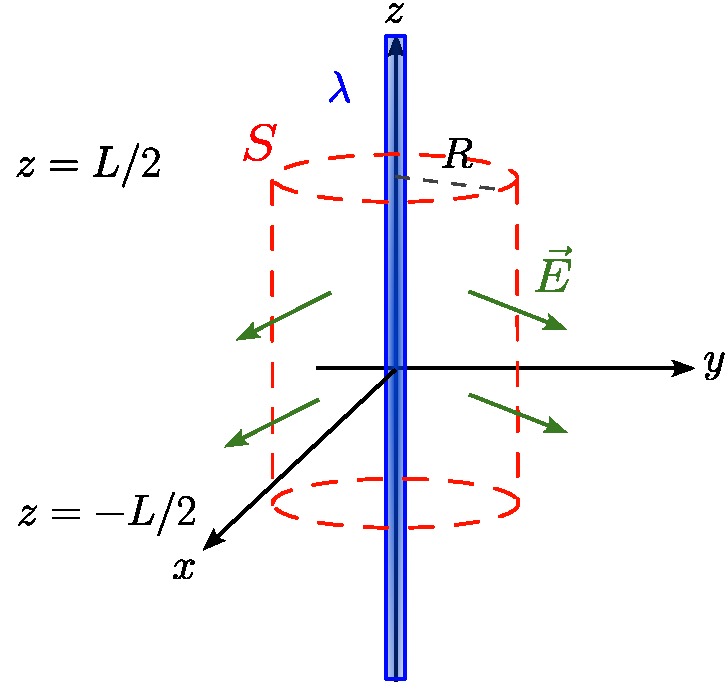
\includegraphics[scale = 0.65]{Figuras/Ej-Gauss-2.pdf}
    \caption{Superficie Gaussiana para un alambre infinito $R$ cargado uniformemente.}
    \label{fig:Ej-Gauss-2}
\end{figure}

\textbf{Solución:} El campo eléctrico del alambre infinito está en la dirección de $\hat{\rho}$, es decir, $\vec{E} = E \hat{\rho}$. Por ello, para aplicar la Ley de Gauss, se utilizará como \textit{superficie Gaussiana} un cilindro centrado en el origen de radio $R$, distancia donde queremos evaluar el campo, la cual el campo tiene módulo constante, y altura $L$ con la  tapa inferior en el plano $z = -L/2$ y la tapa superior en el plano $z = L/2$.

Usando coordenadas cilíndricas, se tiene que

\begin{itemize}
\item $dq = \lambda \,dz $ (diferencial de la carga encerrada),

\item $d\vec{S}_M = R \, d\varphi \,dz \hat{\rho} $ (elemento de superficie del manto).

\item $d\vec{S}_{TI} = - R \,d\varphi\, d\rho \,\hat{k}$ (elemento de superficie de la tapa inferior). 

\item $d\vec{S}_{TS} = R \,d\varphi\, d\rho \,\hat{k}$ (elemento de superficie de la tapa superior).
\end{itemize}

Calculemos
\begingroup
\allowdisplaybreaks
\begin{align*}
    \oiint_S \vec{E} \cdot d\vec{S} &= \iint_{S_{M}} \vec{E} \cdot d\vec{S}_M + \iint_{S_{TI}} \vec{E} \cdot d\vec{S}_{TI} + \iint_{S_{TS}} \vec{E} \cdot d\vec{S}_{TS} \\
    &= \int_{-L/2}^{L/2} \int_0^{2\pi} (E\,\hat{\rho}) \cdot (R\,d\varphi\, dz \,\hat{\rho}) + \cancelto{0}{\int_0^R \int_0^{2\pi} (E\,\hat{\rho})\cdot (- R \,d\varphi \,d\rho \,\hat{k} )} \\
    & \quad + \cancelto{0}{\int_0^R \int_0^{2\pi} (E\,\hat{\rho})\cdot (R \,d\varphi\, d\rho\, \hat{k})} \\
    &= \int_{-L/2}^{L/2} \int_0^{2\pi} E R \,d\varphi \,dz \\
    &= 2\pi L ER.
\end{align*}
\endgroup

Por la ley de Gauss, tenemos que
\begin{align*}
    \oiint_S \vec{E} \cdot d\vec{S} = \frac{q_{encerrada}}{\varepsilon_0} &\Rightarrow 2\pi L E R = \frac{1}{\varepsilon_0} \int_{-L/2}^{L/2} \lambda \,dz = \frac{\lambda L}{\varepsilon} \\
    &\Rightarrow E = \frac{\lambda}{2\pi \varepsilon_0 R}.
\end{align*}

Por lo tanto, generalizando ($R \to \rho$),
$$\Vec{E}(\Vec{x}) = \frac{\lambda}{2\pi \varepsilon_0 \rho} \,\hat{\rho}.$$

\end{ejemplo}

\begin{ejemplo}[Propuesto]
Determinar el campo electrostático  de un plano infinito en el plano $xy$. 

\textbf{Hint:} Tomar como superficie Gaussiana un cilindro centrado en el origen tal que el plano divida al cilindro en dos. 

\textbf{Solución:}  $\vec{E} = \frac{\sigma}{2\varepsilon_0} \,\hat{k}$ para $z > 0$ y $\vec{E} = - \frac{\sigma}{2 \varepsilon_0} \,\hat{k}$ para $z <0$.

\end{ejemplo}


\subsection{Forma diferencial de la ley de Gauss}

La ley de Gauss (para  la electrostática) está dada por
$$\oiint_S \vec{E} \cdot d\vec{S} = \frac{q}{\varepsilon_0}.$$

Para cargas distribuidas en un volumen, podemos escribir la carga por
$$q = \iiint_V \rho(\vec{x}) \,dV.$$

Luego, 
$$\oiint_S \vec{E} \cdot d\vec{S} = \frac{1}{\varepsilon_0} \iiint_V \rho(\vec{x}) \,dV.$$

Por el teorema de Gauss (de la divergencia), tenemos que
$$\oiint_S \vec{E} \cdot d\vec{S} = \iiint_V \vec{\nabla} \cdot \vec{E} \,dV$$ 

Por transitividad, 
\begin{equation*}
\iiint_V \frac{1}{\varepsilon_0} \rho (\vec{x}) d V =   \iiint_V \vec{\nabla} \cdot \vec{E} \,dV.
\end{equation*}

Así, hemos probado que \textcolor{red}{para todo volumen} $V$, se verifica
$$\iiint_V \left( \frac{1}{\varepsilon_0} \rho (\vec{x}) - \vec{\nabla} \cdot \vec{E}  \right) \, dV= 0.$$


Por lo tanto, se obtiene ecuación
\begin{shaded}
$$\vec{\nabla} \cdot \vec{E} = \frac{\rho(\vec{x})}{\varepsilon_0},$$    
\end{shaded}

conocida como la \textbf{primera ecuación de Maxwell}.

